\documentclass[]{../metanetpaper}

%!TEX TS-program = xelatex
\RequireXeTeX %Force XeTeX check


\title{Languages in the European Information Society}
\date{\today}
\author{Dr. John Doe (DFKI), Prof. Dr. Felix Sasaki (DFKI),\\
        Pepe Pérez (Academia de \LaTeX), Tan Ah Kao (USEV)}


\begin{document}

	\maketitle

	\section*{Preface}
This white paper is part of a series that promotes knowledge about
language technology and its potential. It addresses educators, journalists, politicians, language communities and others. The availability and use of language technology in Europe varies between languages. Consequently, the actions that are required to further support research and development of language technologies also differ for each language. The required actions depend on many factors, such as the complexity of a given language and the size of its community.
META-NET, a Network of Excellence funded by the European Commission, has conducted an analysis of current language resources and technologies. This analysis focused on the 23 official European languages as well as other important national and regional languages in Europe. The results of this analysis suggest that there are many significant research gaps for each language. A more detailed expert analysis and assessment of the current situation will help maximise the impact of additional research and minimize any risks. META-NET consists of 47 research centres from 31 countries that are working with stakeholders from commercial businesses, government agencies, industry, research organisations, software companies, technology providers and European universities. Together, they are creating a common technology vision while developing astrategic research agenda that shows how language technology applications can address any research gaps by 2020.

\clearpage

	\tableofcontents

	% 1.
	\clearpage
	\section{Executive Summary --- Zusammenfassung}
	

Many European languages run the risk of becoming victims of the digital age because they are underrepresented and underresourced online. Huge regional market opportunities remain untapped today because of language barriers. If we do not take action now, many European citizens will become socially and economically disadvantaged because they speak their native language. Innovative language technology is an intermediary that will enable European citizens to participate in an egalitarian, inclusive and economically successful knowledge and information society. Multilingual language technology will be a gateway for instantaneous, cheap and effortless communication and interaction across language boundaries. Today, language services are primarily offered by commercial providers from the US. Google Translate, a free service, is just one example. The recent success of Watson, an IBM computer system that won an episode of the Jeopardy game show against human candidates, illustrates the immense potential of language technology. As Europeans, we have to ask ourselves several urgent questions:
\\
\begin {itemize}
\item Should our communications and knowledge infrastructure be dependent upon monopolistic companies?
\item Can we truly rely on language-related services that can be immediately switched off by others?
\item Are third parties from other continents willing to address our translation problems and other issues that relate to European multilingualism?
\item Can our European cultural background help shape the knowledge society by offering better, more secure, more precise, more innovative and more robust high-quality technology?
\end {itemize}
This whitepaper for the German language demonstrates that a language technology research and development community exists in Germany, Austria and Switzerland. However, many large companies have stopped their activities in language technology research and development, which is nowadays almost exclusively performed by small and medium enterprises that can hardly compete on the global market. While Germany used to be a European hub in this area in the past, we now have to ask ourselves if we want to actively compete in the global market for research and development in this
future technology or not. Although a number of technologies and resources for Standard German exist, there are fewer technologies and resources for the German language than for the English language. The existing tech nologies and resources are also poorer in quality. According to the assessment detailed in this report, immediate
action must occur before any breakthroughs for the German language can be achieved.

	\section{Risk for Our Languages and a Challenge for Language Technology}

We are witnesses to a digital revolution that is dramatically impacting communication and society.
	\margin{We are currently witnessing a digital revolution that is comparable to Gutenberg’s invention of the
	printing press.}
Recent developments in digitalinformation and communication technology are sometimes compared to Gutenberg’s invention of the printing press. What can this analogy tell us about the future of the European information society and our languages in particular?\\
After Gutenberg’s invention, real breakthroughs in communication and knowledge exchange were accomplished by efforts such as Luther’s translation of the Bible into vernacular language. In subsequent centuries, cultural techniques have been developed to better handle language processing and knowledge exchange:
\begin{itemize}
\item the orthographic and grammatical standardisation of major languages enabled the rapid dissemination of new scientific and intellectual ideas;
\item the development of official languages made it possible for citizens to communicate within certain (often political) boundaries;
\item the teaching and translation of languages enabled exchanges across languages;
\item the creation of editorial and bibliographic guidelines assured the quality and availability of printed material;
\item the creation of different media like newspapers, radio, television, books, and other formats satisfied different communication needs. In the past twenty years, information technology has helped to automate and facilitate many of the processes:
\item desktop publishing software has replaced typewriting and type setting;
\item Microsoft PowerPoint has replaced overhead projector transparencies;
\item e-mail send and receive documents faster than a fax machine;
\item Skype offers cheap Internet phone calls and hosts virtual meetings;
\item audio and video encoding formats make it easy to exchange multimedia content;
\item search engines provide keyword-based access to web pages;
\item online services like Google Translate produce quick, approximate translations;
\item social media platforms such as Facebook, Twitter, and Google+ facilitate communication, collaboration, and information sharing.
\end{itemize}
Although such tools and applications are helpful, they are not yet capable of supporting a sustainable, multilingual European society for all where information and goods can flow freely.
	
	\subsection{Language Borders Hinder the European Information Society}
We cannot predict exactly what the future information society will look like. But there is a strong likelihood that the revolution in 6 communication technology is bringing people speaking different languages together in new ways. This is putting pressure on individuals to learn new languages and especially on developers to create new technology applications to ensure mutual understanding and access to shareable knowledge.
	\margin{A global economy and information space confronts us with more languages, speakers and content.}
In a global economic and information space, more languages, speakers and content interact more quickly with new types of media. The current popularity of social media (Wikipedia, Facebook, Twitter, YouTube, and, recently, Google+) is only the tip of the iceberg. Today, we can transmit gigabytes of text around the world in a few seconds before we recognize that it is in a language we do not understand. According to a recent report from the European Commission, 57\% of Internet users in Europe purchase goods and services in languages that are not their native language. (English is the most common foreign language followed by French, German and Spanish.) 55\% of users read content in a foreign language while only 35\% use another language to write e-mails or post comments on the Web.i A few years ago, English might have been the lingua franca of the Web — the vast majority of content on the Web was in English — but the situation has now drastically changed. The amount of online content in other European (as well as Asian and Middle
Eastern) languages has exploded. Surprisingly, this ubiquitous digital divide due to language borders has not gained much public attention; yet, it raises a very pressing question: Which European languages will thrive in the networked
information and knowledge society, and which are doomed to disappear?

	\subsection{Our Languages at Risk}
	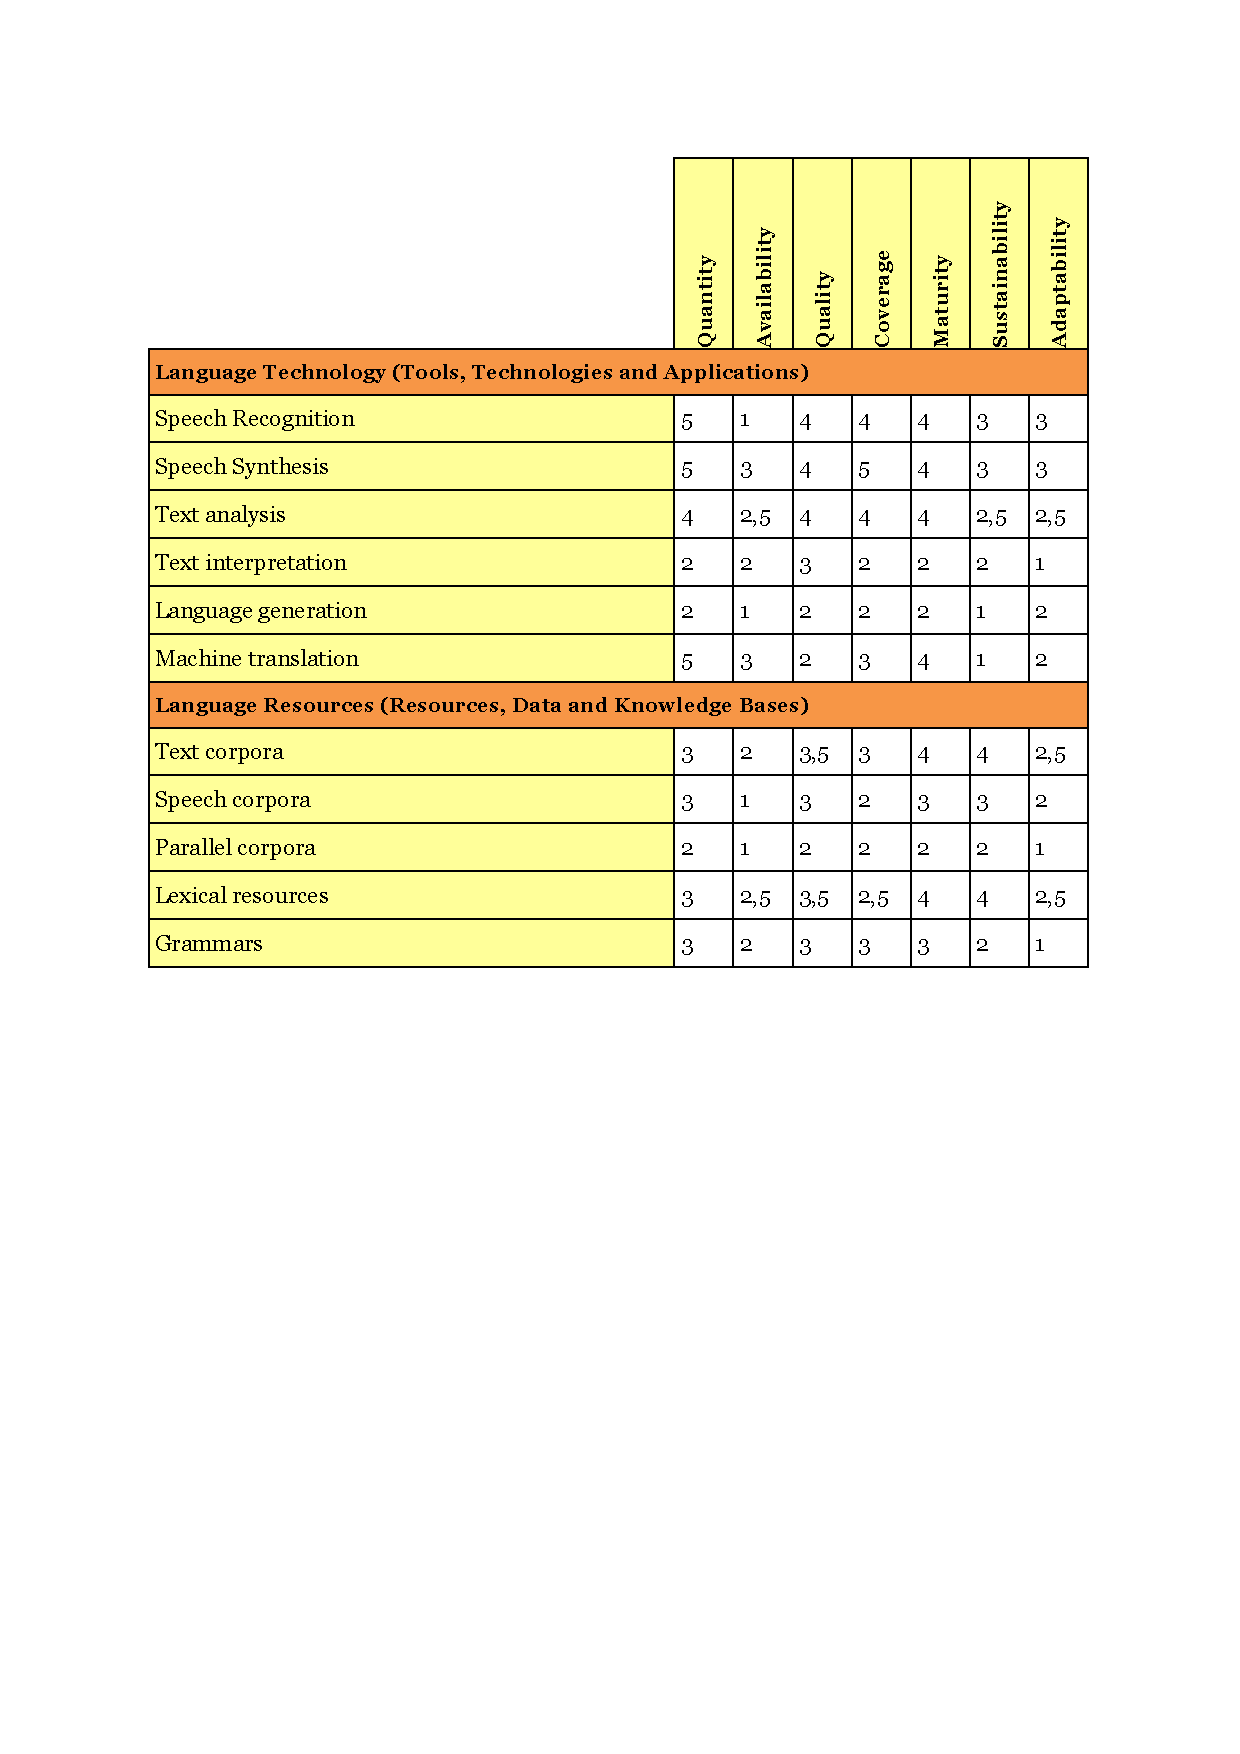
\includegraphics[scale=0.75]{media/metanet-paper2.pdf} 
\\While the printing press helped step up the exchange of information in Europe, it also led to the extinction of many European languages. Regional and minority languages were rarely printed and languages such as Cornish and Dalmatian were limited to oral forms of transmission, which in turn restricted their scope of use. Will the Internet have the same impact on our languages? Europe’s approximately 60 languages are one of its richest and most important cultural assets, and a vital part of its unique social model.\footnote{European Commission, Multilingualism: an asset for Europe and a shared commitment, Brussels, 2008 (http://ec.europa.eu/education/languages/pdf/com/2008\_0566\_en.pdf).}
\margin{The wide variety of languages in Europe is one of its richest and most important cultural assets.} While languages such as English and Spanish are likely to survive in the emerging digital marketplace, many European languages could become irrelevant in a networked society. This would weaken Europe’s global standing, and run counter to the strategic goal of ensuring equal participation for every European citizen regardless of language. According to a UNESCO report on multilingualism, languages are an essential medium for the enjoyment of fundamental rights, such as political expression, education and participation in society.\footnote{UNESCO Director-General, Intersectoral mid-term strategy on languages and multilingualism, Paris, 2007 (http://unesdoc.unesco.org/images/0015/001503/150335e.pdf).}

	\subsection{Language Technology is a Key Enabling Technology}
In the past, investment efforts in language preservation focused on language education and translation. According to one estimate, the European market for translation, interpretation, software localisation and website globalisation was €8.4 billion in 2008 and is expected to grow by 10\% per annum.iv Yet this figure covers just a small proportion of current and future needs in communicating between languages. \margin {Language technology helps people collaborate, conduct business, share knowledge and participate in social and political debates across differ} The most compelling solution for ensuring the breadth and depth of language usage in Europe tomorrow is to use appropriate technology, just as we use technology to solve our transport, energy and disability needs among others. Digital language technology (targeting all forms of written text and spoken discourse) helps people collaborate, conduct business, share knowledge and participate in social and political debate regardless of language barriers and computer skills. It often operates
invisibly inside complex software systems to help us:
\begin{itemize}
\item find information with an Internet search engine;
\item check spelling and grammar in a word processor;
\item view product recommendations in an online shop;
\item hear the verbal instructions of a car navigation system;
\item translate web pages via an online service.
\end{itemize}
Language technology consists of a number of core applications that enable processes within a larger application framework. The purpose of the META-NET language white papers is to focus on how ready these core technologies are for each European language.\margin {Europe needs robust and affordable language technology for all European languages.}
To maintain our position in the frontline of global innovation, Europe will need language technology adapted to all European languages that is robust, affordable and tightly integrated within key software environments. Without language technology, we will not be able to achieve a really effective interactive, multimedia and multilingual user experience in the near future.
	
	\subsection{Opportunities for Language Technology}
In the world of print, the technology breakthrough was the rapid duplication of an image of a text (a page) using a suitably powered printing press. Human beings had to do the hard work of looking up, reading, translating, and summarizing knowledge. We had to wait until Edison to record spoken language – and again his technology simply made analogue copies. Digital language technology can now automate the very processes of translation, content production, and knowledge management for all European languages. It can also empower intuitive language/speech-based interfaces for household electronics, machinery, vehicles, computers and robots. Real-world commercial and industrial applications are still in the early stages of development, yet R\&D achievements are creating a genuine window of opportunity. For example, machine translation is already reasonably accurate in specific domains, and experimental applications provide multilingual information and knowledge management as well as content production in many European languages. As with most technologies, the first language applications such as voice-based user interfaces and dialogue systems were developed for highly specialised domains, and often exhibit limited performance. But there are huge market opportunities in the education and entertainment industries for integrating language technologies
into games, cultural heritage sites, edutainment packages, libraries, simulation environments and training programmes. Mobile information services, computer-assisted language learning software, eLearning environments, self-assessment tools and plagiarism detection software are just some of the application areas where language technology can play an important role. The popularity of social media applications like Twitter and Facebook suggest a further need for sophisticated language technologies that can monitor posts, summarise discussions, suggest opinion trends, detect emotional responses, identify copyright infringements or track misuse.

Language technology represents a tremendous opportunity for the European Union. It can help address the complex issue of multilingualism in Europe – the fact that different languages coexist naturally in European businesses, organisations and schools. But citizens need to communicate across these language borders criss-crossing the European Common Market, and language technology can help overcome this final barrier while supporting the free and open use of individual languages. Looking even further forward, innovative European multilingual language technology will provide a benchmark for our global partners when they begin to enable their own multilingual communities. Language technology can be seen as a form of ‘assistive’ technology that helps overcome the ‘disability’ of linguistic diversity and make language communities more accessible to each other. \margin{Language technology helps overcome the “disability” of linguistic diversity.}
Finally, one active field of research is the use of language technology for rescue operations in disaster areas, where performance can be a matter of life and death: Future intelligent robots with cross-lingual language capabilities have the potential to save lives.

	\subsection{Challenges Facing Language Technology}
Although language technology has made considerable progress in the last few years, the current pace of technological progress and product innovation is too slow.\margin{The current pace of technological progress is too slow.} Widely-used technologies such as the spelling and grammar correctors in word processors are typically monolingual, and are only available for a handful of languages. Online machine translation services, although useful for quickly generating a reasonable approximation of a document’s contents, are fraught with difficulties when highly accurate and complete translations are required. Due to the complexity of human language, modelling our tongues in software and testing them in the real world is a long, costly business that requires sustained funding commitments. Europe must therefore maintain its pioneering role in facing the technology challenges of a multiple-language community by inventing new methods to accelerate development right across the map. These could include both computational advances and techniques such as crowdsourcing.

	\subsection{Language Acquisition in Humans and Machines}
To illustrate how computers handle language and why it is difficult to program them to use it, let’s look briefly at the way humans acquire first and second languages, and then see how language technology systems work. 
Humans acquire language skills in two different ways. Babies acquire a language by listening to the real interactions between its parents, siblings and other family members.\margin{Humans acquire language skills in
two different ways: learning examples and learning the underlying language rules.} From the age of about two, children produce their first words and short phrases. This is only possible because humans have a genetic disposition to imitate and then rationalize what they hear. 
Learning a second language at an older age requires more effort, largely because the child is not immersed in a language community of native speakers. At school, foreign languages are usually acquired by learning grammatical structure, vocabulary and spelling using drills that describe linguistic knowledge in terms of abstract rules, tables and examples. Learning a foreign language gets harder with age.
The two main types of language technology systems ‘acquire’ language capabilities in a similar manner.\margin{The two main types of language technology systems acquire language in a similar manner} Statistical (or ‘data-driven’) approaches obtain linguistic knowledge from vast collections of concrete example texts. While it is sufficient to use text in a single language for training, e.g., a spell checker, parallel texts in two (or more) languages have to be available for training a machine translation system. The machine learning algorithm then “learns” patterns of how words, short phrases and complete sentences are translated. 
This statistical approach can require millions of sentences and performance quality increases with the amount of text analysed. This is one reason why search engine providers are eager to collect as much written material as possible. Spelling correction in word processors, and services such as Google Search and Google Translate all rely on statistical approaches. The great advantage of statistics is that the machine learns fast in continuous series of training cycles, even though quality can vary arbitrarily.
The second approach to language technology and machine translation in particular is to build rule-based systems. Experts in the fields of linguistics, computational linguistics and computer science first have to encode grammatical analyses (translation rules) and compile vocabulary lists (lexicons). This is very time consuming and labour intensive. Some of the leading rule-based machine translation systems have been under constant development for more than twenty years. The great advantage of rule-based systems is that the experts have more detailed control over the language processing. This makes it possible to systematically correct mistakes in the software and give detailed feedback to the user, especially when rule-based systems are used for language learning. But due to the high cost of this work, rule-based language technology has so far only been developed for major languages. 
As the strengths and weaknesses of statistical and rule-based systems tend to be complementary, current research focuses on hybrid approaches that combine the two methodologies. However, these approaches have so far been less successful in industrial applications than in the research lab. 
As we have seen in this chapter, many applications widely used in today’s information society rely heavily on language technology. Due to its multilingual community, this is particularly true of Europe’s economic and information space. Although language technology has made considerable progress in the last few years, there is still huge potential in improving the quality of language technology systems. In the following, we will describe the role of German in European information society and assess the current state of language technology for the German language. 
	\clearpage
	
	\section{German in the European Information Society}
	\subsection{General Facts}
With about 100 million native speakers, German is the most widely spoken native language in the European Union. It is the commonly used language in Germany, Austria and Liechtenstein, and it is one of the official languages of Switzerland, Luxembourg and Belgium where it is used by parts of the population. \margin{German is the second most studied foreign language in the EU after English.} Around the world, German is spoken by around 30 million non-native speakers.i German is also the second most studied foreign language in the EU after English.ii 
In Germany, the German language is the common spoken and written language as well as the native language of the vast majority of the population. Minority languages in the sense of the European Charter on Regional and Minority Languages include: Danish and North Frisian in Schleswig-Holstein; Upper Sorbian in Saxony; Lower Sorbian in Brandenburg; Saterland Frisian in Lower Saxony; and the Romani language of the German Roms and Sinti throughout the country. Each group represents some tens to hundreds of thousands of speakers.iii In addition, there are immigrant languages in Germany, such as Turkish, which has roughly 3.3 million speakers.
In Austria and Liechtenstein, German is the official language as well as the most common spoken and written language. In Austria, recognized minority languages include: Slovenian, Croatian (Burgenland-Kroatisch), Slovak, Romani, Hungarian and Czech. Other languages spoken in Austria are Turkish and the languages of former Yugoslavia—Bosnian, Croatian and Serbian.
In Switzerland, German shares its official status with the French, Italian and Rhaeto-Romanic languages. In Belgium, German, Dutch and French are official languages. In Luxembourg, German, French and Luxembourgish are official languages. German variants are also spoken by minorities in other EU countries, such as France (Alsace and Lorraine), Italy (South Tyrol) and Poland (Silesia).
German has a large variety of dialects such as Bavarian and Swabian. By and large, the dialects have the same grammar, although some dialects exhibit slightly different syntactic constructions. The division of Germany into two between 1945 and 1989 is still reflected in some lexical differences, for example, Plastik or Plaste [plastics].
Austrian German (AT) is a variant of German (Oberdeutsch) whose lexicon differs from the official language used in Germany (DE), e.g.: 

\begin{tabular}{ccc}
\hline \textbf{English} & \textbf{Austrian German} & \textbf{Standard German} \\ 
\hline chair & Sessel & Stuhl \\ 
\hline armchair & Fauteuil & Sessel \\ 
\hline Tobacconist & Trafik & Tabakladen \\
\hline
\end{tabular} 
enisation (or consonant weakening) is also widespread in spoken Austrian German. For instance, there is no pronounced phonemic distinction between backen [to bake] and packen [to pack] or Teich [lake] and Deich [dyke]. Unlike in Standard German in Germany, the past tense is rarely used in Austrian German; speakers prefer the perfect tense when expressing past events. 
Swiss German (CH) has borrowed a number of French words such as Velo (CH) instead of Fahrrad (DE) for bicycle. There are also some morphological and orthographical variations.i For example, ss is used instead of ß and some words are spelled differently, for example, Müesli (CH) instead of Müsli (DE) for cereal. Multilingualism is a matter of course in Switzerland with its four official languages.

	\subsection{Particularities of the German Language}
German exhibits a number of specific characteristics that contribute to the richness of the language but can also be a challenge for the computational processing of natural language. For instance, speakers can express the same idea in a wide variety of ways.
First, word order is relatively free in German sentences. The following sentence in English:
\begin{center}
\textit{The woman gave the man an apple.}
\end{center}
can also be expressed in two other ways:
\begin{center}
\textit{The woman gave an apple to the man.}\\
\textit{An apple was given to the man by the woman.}
\end{center}
In German, however, there are at least nine possible ways to express the same sentence, although some of them are very rarely used.
\begin{center}
\textit{Die Frau gab dem Mann einen Apfel.\\
Einen Apfel gab die Frau dem Mann.\\
Dem Mann gab die Frau einen Apfel.\\
Ein Apfel wurde dem Mann von der Frau gegeben.\\
Dem Mann wurde von der Frau ein Apfel gegeben.\\
Dem Mann wurde ein Apfel von der Frau gegeben.\\
Ein Apfel wurde von der Frau dem Mann gegeben.\\
Von der Frau wurde dem Mann ein Apfel gegeben.\\
Von der Frau wurde ein Apfel dem Mann gegeben.}
\end{center}
Second, German is extremely productive when it comes to coining new words. This is mainly due to the compounding system that allows speakers to combine words and affixes in a fairly simple way. In theory, this allows for the creation of infinitely long words:
\begin{center}
\textit{Verteidigung (defence)\\
Verteidigungsminister (minister of defence)\\
Selbstverteidigungsminister (minister of self-defence)\\
Bundesselbstverteidigungsminister (federal minister of self-defence)}
\end{center}
Humans can easily derive the meanings of these neologisms as above, but machines have difficulty processing them. 
There are other specific characteristics of the German language that make it hard to process with a computer. One is a tendency to use fairly long, nested sentences. Another is the ability to position separable verb prefixes far away from their associated verb. For example, the verb vorstellen can be found in sentences such as:
\begin{center}
\textit{Er \textbf{stellte} sich, nachdem er mir ein Getränk angeboten hatte und wir ins Gespräch gekommen waren, \textbf{vor}.\\
(He introduced himself after he had offered me a drink and we had started a conversation.)}
\end{center}
The meaning of verbs that can “take” different prefixes, such as vor, ein or aus, is often confusing for German language learners. For example: the verb stellen [to put] changes its meaning in vorstellen [imagine or introduce], einstellen [hire, discontinue or regulate], or ausstellen [exhibit, switch off or issue].

	\subsection{Recent Developments}
Starting in the 1950s, American television series and movies began to dominate the German market. Although foreign films and series are usually dubbed into German (unlike countries such as Sweden and Poland), the strong presence of the American way of life in the media had an influence on popular German culture and language. Due to the continuing triumph of English and American music since the 1960s, generations of Germans have been widely exposed to English during their adolescence. English soon acquired the status of a cool and hip language, and this continues today.
The continued popularity of English is reflected in the sheer number of loan words from the English language (Anglicisms). A systematic investigation of neologisms in German newspapers since 2000 revealed that about one third of the neologisms are complete or partial Anglicisms.i In most cases the words fill a vocabulary gap—they complement native German words rather than competing with them. However, Anglicisms have started to replace existing German vocabulary in some areas. The use of English titles in job advertisements is one example, especially for executive positions (e.g., “Human Resource Manager” instead of Personalleiter). Product advertisements also have a strong tendency to overuse Anglicisms. In 2003, Endmark conducted a study of the use of English advertising slogans by German companies. The study revealed that almost all of the 12 slogans investigated were misunderstood by more than half of the respondents; as a result the companies replaced them with German equivalents. This example demonstrates how important it is to raise awareness about the risk of excluding large parts of the population from participating fully in the information society, especially those who are less familiar with English. Translations or explanations should be made available where necessary.
	\subsection{Language Cultivation in Germany}
Germany has no institutional body responsible for developing or implementing a policy to protect the German language. However, there are a number of non-governmental, publicly-funded organisations that play an active role in the promotion of the German language. The Goethe Institute works in partnership with the Federal Foreign Office.\margin{Germany has no institutional body responsible for developing or implementing potential language protection policies.} The institute offers German language courses all over the world in order to strengthen the international standing of the German language. Other organisations that raise awareness about the German language and promote German language culture in Germany include the German Academy for Language and Literature (DASD) and the Society for the German Language (GfDS), which has been charged by the German Bundestag (Federal Parliament) with controlling the language of legislative texts. The Institute for the German Language (IDS) is the central research centre for German. 
In addition, individual authors contribute to linguistic awareness by discussing undesirable developments such as the widespread use of incorrect apostrophes (Maria’s Haus instead of the correct Marias Haus), business jargon and neologisms. The best-known author of this type is Bastian Sicki and his magazine column "Zwiebelfisch".ii Private initiatives usually target Anglicisms: the Verein Deutsche Sprache (VDS) initiative annually awards its Kulturpreis Deutsche Sprache [cultural prize for the German language] for creative contributions to the development of the German language. (In 2011, Udo Lindenberg, a German singer, won the award.) The Aktion lebendiges Deutsch [action for lively German] campaign regularly organizes contests to Germanize egregious Anglicisms. 
Germany does not have a language academy that advises on preferred language usage unlike the Académie Francaise in France or the Academía Real in Spain. The Duden dictionary used to be a prescriptive source for German spelling and grammar, but it now takes a more descriptive approach.iii 
Political measures to influence or modify the German language are rare.\margin{Political measures focused on the German language are rare. After 10 years’ of discussion, Austria, Germany, Liechtenstein and Switzerland agreed on a spelling reform in 2006.} After 10 years’ of discussion, Austria, Germany, Liechtenstein and Switzerland agreed on a spelling reform in 2006. The original reform was modified and weakened, and it gave writers more freedom. The new spelling conventions were not accepted universally; many large newspapers and publishers use a mixture of old and new spelling conventions (house spelling rules).
There are almost no measures designed to protect the official status of the German language. In December 2008, several politicians and private associations (most notably the VDS) called for a change to the constitution that would add a clause making German the official language of the Federal Republic of Germany. This was rejected by the German Bundestag but is still a hot topic. In 2004, the government considered but failed to introduce a quota for radio stations (like that found in France) on how much music must be sung in German. 
The above examples illustrate the disadvantageous situation of the German language when compared, for example, to French, which gets strong financial backing from the global community of French speakers (Francophonie). The comparably low level of cultural identity associated with the contemporary German language certainly encourages an attitude of tolerance and openness towards cultural diversity, but it can also pose a threat to maintaining a certain standard of expressivity for German.

	\subsection{Language in Education}
The first study published by the OECD Programme for International Student Assessment (PISA) in 2000 revealed that German students had below average reading literacy. Students from immigrant families had particularly poor results. The ensuing debate increased public awareness about the importance of language learning, especially for socially integrating immigrants. 
Using the recommendations of the OECD, Germany has adopted several laws on early language training in the last decade. One example is the Gesetz zur vorschulischen Sprachförderung [Law for the Promotion of Pre-School Language Learning], which came into effect in April 2008 in Berlin, a city with a very high number of children whose native language is not German. (This means more than 90\% of the children in some parts of the Neukölln district). The law introduces a compulsory German test for children who did not attend kindergarten before enrolling in school, and provides enhanced language training for those that have insufficient German language skills.
Measures such as the language law in Berlin have been successful, as the 2009 PISA study showed that reading literacy among Germans had significantly improved since 2000, in particular for children from immigrant families. However, there are still major differences in language skills between students with and without a native-language background compared to other countries with a similar situation.i The differences are particularly salient in Austria, which is among the three OECD countries that show the widest gap between native and immigrant skills in reading literacy among young people.
The use of the German language has become critical to immigration policy in Germany. The law on controlling and limiting immigration as well as regulating the residence and integration of migrants that came into force in 2005 puts a special emphasis on the need to learn German in integration classes. These classes include 600 hours of language teaching plus a 30-hour introduction to German history, culture and law. Immigrants who do not participate in these integration classes may have their state benefits reduced, or encounter difficulties when they renew their residence permits. Participation in the classes is also a prerequisite for obtaining permanent residency in Germany.
Language skills are a key qualification for education and personal and professional communication.\margin{Language skills are a key qualification for education and for personal and professional communication. Yet German plays a relatively minor role as a school subject in secondary education. } Yet, German plays a relatively minor role as a school subject in secondary education. According to OECD figures published in 2003, German language instruction forms about 20\% of the school curriculum for nine to eleven year old pupils, compared with almost 33\% native language instruction in France, Greece and the Netherlands. ii
Increasing the amount of German language instruction in schools is one possible step towards providing students with the language skills they require for active participation in society. Language technology can make an important contribution in this respect by offering so-called computer-assisted language learning (CALL) systems that allow students to experience language in an attractive way, for example, by linking vocabulary in electronic texts to easy-to-understand definitions or to audio or video files that supply additional information such as pronunciation. 

	\subsection{International Aspects}
Germany is often referred to as the land of Dichter und Denker [poets and thinkers] due to its immense contributions to literature, philosophy and science. The works of authors such as Goethe, Kafka and Hesse have gained international fame; the philosophical ideas of Kant, Hegel, Marx and Nietzsche as well as Freud's theory of psychoanalysis have made a lasting impact on modern culture. Scientists from German-speaking countries have won numerous Nobel Prizes in literature, economy, physics, chemistry and medicine.
At the beginning of the 20th century,\margin{At the beginning of the 20th century, German-speaking countries were at the forefront of scientific disciplines, and German was the major scientific language—30\% of scientific publications were written in German. Since then, the importance of German as a scientific language has dramatically decreased.} German-speaking countries were at the forefront of scientific disciplines, and German was the major scientific language—30\% of scientific publications were written in German. Since then, the importance of German as a scientific language has dramatically decreased and less than 5\% of scientific publications are currently written in German—most of them in disciplines such as law, philosophy and theology.i This situation can only partly be attributed to a decline in scientific contributions from German-speaking countries. Even in the universities of these countries, German is strongly challenged or has even been overtaken by English as the language of publication in many disciplines.
The same goes for the business world. In many large companies operating across borders, English has become the lingua franca for written (e-mails and documents) and oral communication (presentations and meetings). Such developments strongly affect the status of German as a foreign language. Pragmatic reasons for learning German, such as better job market chances, have lost their importance, and German is losing more ground to English and recently to Chinese. 
In the European Union,\margin{German is one of the three official working languages of the European Commission, but it is hardly used in the EU’s official business.} German is one of the three official working languages of the European Commission (along with English and French), but in practice, German is hardly used in the EU’s official business. Only 3\% of the documents sent by the European Commission to the Member States are written in German.ii Recently political action was taken to address this problem. In 2006, Norbert Lammert, the President of the German Bundestag, wrote a letter to the European Commission saying that the German Bundestag will reject contracts and similar documents if a German translation is not available. Language technology can address this challenge by offering services such as machine translation or cross-lingual information retrieval. Such technologies can help diminish the personal and economic disadvantages facing non-native English speakers in Europe.
	
	\subsection{German on the Internet}
In 2010, almost 70% of the German population and 74.8% of the Austrian population were Internet users and most said they were online every dayi. The percentage of young people using the Internet is even higher in both countries. The strong presence of German on the Web is also mirrored by the fact that the German Wikipedia is the second largest Wikipedia after English (not including automatically translated versions like the Thai Wikipedia).
With about 14 million Internet domains in November 2010, the .de top-level country domain for Germany is the world’s largest country extension, and it is the second largest extension after the .com domain.ii This dominant Internet presence suggests that there is a vast amount of German language data on the Web. In addition, some bilingual resources such as the LEO online dictionary are available for free. iii
The growing importance of the Internet is critical for language technology. The vast amount of digital language data is a key resource for analysing the usage of natural language, in particular, for collecting statistical information about patterns. And the Internet offers a wide range of application areas for language technology. 
The most commonly used web application is search, which involves the automatic processing of language on multiple levels as will be shown in more detail later. Web search involves sophisticated language technology that differs for each language. For the German language, for example, this involves matching ä and ae, or taking capitalization into account to distinguish between nouns and verbs, for example, Fliegen [flies] and fliegen [to fly]. 
One important aspect of equal opportunities in Germany and other European countries is the Gesetz zur Gleichstellung behinderter Menschen [Law on Equal Opportunities for the Disabled], which came into force in 2002, and addresses the issue of Barrierefreie Informationstechnik [barrier-free information technology]. It enjoins public agencies to make sure that the disabled can use their websites and Internet services without any restrictions. User-friendly language technology tools are a key solution to this requirement by offering for example speech synthesis to enunciate the content of web pages for the blind.
Internet users and providers of web content can also use language technology in less obvious ways, for example, by automatically translating web page contents from one language into another. Despite the high cost of manually translating this content, comparatively little language technology has been developed and applied to the issue of website translation in light of the supposed need. This may be due to the complexity of the German language and to the range of different technologies involved in typical applications. 
The next chapter gives an introduction to language technology and its core application areas, together with an evaluation of current language technology support for German. 
	
	\subsection{Language Technology Support for German}
Language technologies are software systems designed to handle human language and are therefore often called “human language technology”. Human language comes in spoken and written forms.\margin{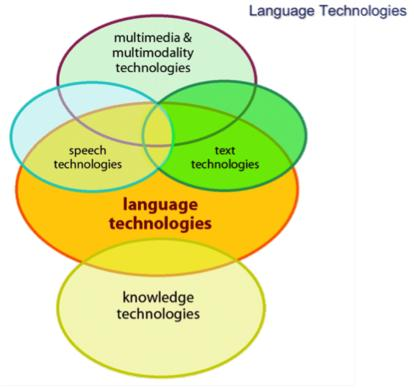
\includegraphics[scale=0.2]{media/test.jpg}  } While speech is the oldest and in terms of human evolution the most natural form of language communication, complex information and most human knowledge is stored and transmitted in written texts. Speech and text technologies process or produce these different forms of language, though they both use dictionaries and rules of grammar and semantics. This means that language technology (LT) links language to various forms of knowledge, independently of the media (speech or text) it is expressed in. The figure on the right illustrates the LT landscape. When we communicate, we combine language with other modes of communication and information media – for example speaking can involve gestures and facial expressions. Digital texts link to pictures and sounds. Movies may contain language in spoken and written form. In other words, speech and text technologies overlap and interact with other technologies that facilitate processing of multimodal communication and multimedia documents. 
In the following, we will discuss the main application areas of language technology, i.e., language checking, web search, speech interaction, and machine translation. This includes applications and basic technologies such as 
\begin{itemize}
\item spelling correction
\item authoring support
\item computer-assisted language learning
\item information retrieval 
\item information extraction
\item text summarization
\item question answering
\item speech recognition 
\item speech synthesis 
\end{itemize}
\margin{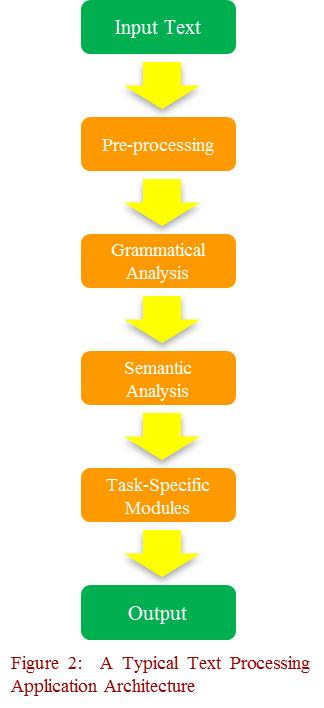
\includegraphics[scale=0.2]{media/page20_2.jpg} }
	
	\subsection{Application Architectures}
Software applications for language processing typically consist of several components that mirror different aspects of language. The figure on the right shows a highly simplified architecture that can be found in a typical text processing system. The first three modules handle the structure and meaning of the text input:
\begin{enumerate}
\item Pre-processing: cleans the data, analyses or removes formatting, detects the input language, replaces ä with ae in German texts, and so on.
\item Grammatical analysis: finds the verb, its objects, modifiers and other parts of speech as well as detects the sentence structure.
\item Semantic analysis: performs disambiguation (i.e., computes the appropriate meaning of words in a given context); resolves anaphora (i.e., which pronouns refer to which nouns in the sentence) and substitute expressions; and represents the meaning of the sentence in a machine-readable way.
\end{enumerate}
After analysing the text, task-specific modules can perform other operations, such as automatic summarization and database look-ups. This is a simplified and idealised description of the application architecture and illustrates the complexity of LT applications. 
After introducing the core application areas for language technology, we shall provide a brief overview of the state of LT research and education today, and end with an overview of past and present research programmes. We shall then present an expert estimate of core LT tools and resources in terms of various dimensions such as availability, maturity and quality. The general situation of LT for the German language is summarized in a table.

	\subsection{Core Application Areas}
n this section, we focus on the most important LT tools and resources, and give an overview of LT activities in Germany, Austria and Switzerland. Tools and resources that are underlined in the text can also be found in the table at the end of this chapter.  
	
		\subsubsection{Language Checking}
Anyone who has used a word processor such as Microsoft Word knows that it has a spelling checker that highlights spelling mistakes and proposes corrections. The first spelling correction programs compared a list of extracted words against a dictionary of correctly spelled words. Today these programs are far more sophisticated. Using language-dependent algorithms for text analysis, they detect errors related to morphology (e.g., plural formation) as well as syntax–related errors, such as a missing verb or a conflict of verb-subject agreement (e.g., she *write a letter). But most spell checkers will not find any errors in the following text: 
\begin{center}

\textit{Eye have a spelling chequer,\\
It came with my Pea Sea.\\
It plane lee marks four my revue\\
Miss Steaks I can knot sea}
\end{center}	
Handling these kinds of errors usually requires an analysis of the context. For example: whether a word needs to be capitalized in German or not:
\begin{center}
\textit{Sie übersetzte den Text ins Englische.\\
(She translated the text into English.)\\
Er las das englische Buch.\\
(He read the English book.)}
\end{center}
This type of analysis either needs to draw on language-specific grammars laboriously coded into the software by experts, or on a statistical language model. In this case, a model calculates the probability of a particular word as it occurs in a specific position (e.g., between the words that precede and follow it). For example: englische Buch is a much more probable word sequence than Englisch Buch. A statistical language model can be automatically created by using a large amount of (correct) language data (called a text corpus). Most of these two approaches have been developed around data from English. Neither approach can transfer easily to German because the language has a flexible word order, unlimited compound building and a richer inflection system. 
Language checking is not limited to word processors; it is also used in “authoring support systems”, i.e., software environments in which manuals and other documentation are written to special standards for complex IT, healthcare, engineering and other products. Fearing customer complaints about incorrect use and damage claims resulting from poorly understood instructions, companies are increasingly focusing on the quality of technical documentation while targeting the international market (via translation or localization) at the same time. Advances in natural language processing have led to the development of authoring support software, which helps the writer of technical documentation use vocabulary and sentence structures that are consistent with industry rules and (corporate) terminology restrictions.
There are a number of German companies and language service providers offering products in this area. Siemens investigated approaches for German and developed the Siemens-Dokumentationsdeutsch, a controlled language for German.i IAI, a German research institute, developed a checking module, CLAT, for German grammar and style. Acrolinx, a German company, offers software with a highly adaptable language checker as well as a terminology database. The acrolinx style guidelines for technical documentation advise against using complex noun compounds like Achsmesshebebühne [hydraulic platform for measuring axles] and metaphorical language like blitzschnell [fast as lightning] or Faustregel [rule of thumb]. The guidelines also discourage the use of man, the impersonal pronoun, for example, Danach stellt man die Maschine aus [afterwards, one switches off the engine)]. Long and nested sentences are also discouraged. This is largely because such bloated language phenomena are hard for humans to process quickly and accurately. They may also be hard for MT systems to translate effectively.
Besides spell checkers and authoring support, language checking is also important in the field of computer-assisted language learning. And language checking applications also automatically correct search engine queries, as found in Google's Did you mean… suggestions. 

	\subsection{Web Search}
Searching the Web, intranets or digital libraries is probably the most widely used yet largely underdeveloped language technology application today. The Google search engine, which started in 1998, now handles about 80% of all search queries.i Since 2004, the verb googeln even has an entry in the Duden dictionary. The Google search interface and results page display has not significantly changed since the first version. Yet in the current version, Google offers spelling correction for misspelled words and  has now incorporated basic semantic search capabilities that can improve search accuracy by analysing the meaning of terms in a search query context.ii The Google success story shows that a large volume of available data and efficient indexing techniques can deliver satisfactory results for a statistically-based approach.  
For more sophisticated information requests, it is essential to integrate deeper linguistic knowledge for text interpretation. Experiments using lexical resources such as machine-readable thesauri or ontological language resources (e.g., WordNet for English or GermaNet for German) have demonstrated improvements in finding pages using synonyms of the original search terms, such as Atomkraft [atomic energy], Kernenergie [atomic power] and Nuklearenergie [nuclear energy], or even more loosely related terms. 
The next generation of search engines will have to include much more sophisticated language technology, in particular in order to deal with search queries consisting of a question or other sentence type rather than a list of keywords. For the query, “Give me a list of all companies that were taken over by other companies in the last five years,” the LT system needs to analyse the sentence syntactically and semantically as well as provide an index to quickly retrieve relevant documents. A satisfactory answer will require syntactic parsing to analyse the grammatical structure of the sentence and determine that the user wants companies that have been acquired, not companies that acquired other companies. For the expression last five years, the system needs to determine the relevant years. And, the query needs to be matched against a huge amount of unstructured data to find the piece or pieces of relevant information the user wants. This is called “information retrieval”, and involves searching and ranking relevant documents. To generate a list of companies, the system also needs to recognize a particular string of words in a document as a company name, a process called “named entity recognition”.
A more demanding challenge is matching a query in one language with documents in another language. Cross-lingual information retrieval involves automatically translating the query into all possible source languages and then translating the results back into the target language. 
Now that data is increasingly found in non-textual formats, there is a need for services that deliver multimedia information retrieval by searching images, audio files and video data. In the case of audio and video files, a speech recognition module must convert the speech content into text (or into a phonetic representation) that can then be matched against a user query.
In Germany, small and medium-sized enterprises such as Neofonie have successfully developed and applied search technologies, delivering the first German web search engine (Fireball) in 1997. It was later bought and further developed as a content portal by Lycos Europe. Today, only a few German companies such as Neofonie or Attensity Group (formerly Empolis) provide their own search engines. Open source technologies like Lucene and Solr are often used by search-focused companies to provide a basic search infrastructure. Other search-based companies rely on international search technologies such as FAST (a Norwegian company acquired by Microsoft in 2008) or the French company Exalead.
These companies focus their development on providing add-ons and advanced search engines for special interest portals by using topic-relevant semantics. Due to the constant high demand for processing power, such search engines are only cost-effective when handling relatively small text corpora. The processing time is several thousand times higher than that needed by a standard statistical search engine like Google. These search engines are in high demand for topic-specific domain modelling, but they cannot be used on the Web with its billions and billions of documents.
MetaGer is a meta search engine run by the University of Hannover. Intrafind, a Munich-based company, and others specialize in intranet search applications and search applications for products like SAP, which require customization for specific customer data. In Switzerland, Eurospider provides information search for internet portals. In Austria, there are web search engines directed only at Austrian sites such as AT:SEARCH, AUSTRIA-SEEK or AUSTROLINKS but their coverage and outreach is fairly limited. In addition to these search engines, Austrian companies have also developed special purpose search engines such as 123people, a real-time people search engine that supports regional and international searches for, e.g., Austria, Germany, Canada, the USA, and the UK, or Tripwolf, an online travel platform. 

	\subsection{Speech Interaction}
Speech interaction technology is used to create interfaces that enable users to interact in spoken language instead of a graphical display, keyboard and mouse. Today, voice user interfaces (VUI) are usually used for partially or fully automated telephone services provided by companies to customers, employees or partners. Business domains that rely heavily on VUIs include banking, supply chain, public transportation, and telecommunications. Other uses of speech technology include interfaces to car navigation systems and the use of spoken language as an alternative to the graphical or touch-screen interfaces in smartphones. 
Speech interaction comprises four technologies:
\begin{enumerate}
\item Automatic speech recognition (ASR) determines which words are actually spoken in a given sequence of sounds uttered by a user.
\item Natural language understanding analyses the syntactic structure of a user’s utterance and interprets it according to the system in question.
\item Dialogue management determines which action to take given the user input and system functionality.
\item Speech synthesis (text-to-speech or TTS) transforms the system’s reply into sounds for the user.
\end{enumerate}
One of the major challenges of ASR systems is to accurately recognise the words a user utters. This means restricting the range of possible user utterances to a limited set of keywords, or manually creating language models that cover a large range of natural language utterances. Using machine learning techniques, language models can also be generated automatically from speech corpora, i.e., large collections of speech audio files and text transcriptions. Restricting utterances usually forces people to use the voice user interface in a rigid way and can damage user acceptance; but the creation, tuning and maintenance of rich language models will significantly increase costs. VUIs that employ language models and initially allow a user to express their intent more flexibly — prompted by a How may I help you? greeting — tend to be automated and are better accepted by users. 
Companies tend to use pre-recorded utterances by professional speakers for generating the output of the voice user interface. For static utterances where the wording does not depend on particular contexts of use or personal user data, this can deliver a rich user experience. But more dynamic content in an utterance may suffer from unnatural intonation because bits of audio files have simply been strung together. Today’s TTS systems are getting better (though they can still be optimized) at producing natural-sounding dynamic utterances.  
Interfaces in the market for speech interaction technology have been considerably standardised during the last decade in terms of their various technology components. There has also been strong market consolidation in speech recognition and speech synthesis. The national markets in the G20 countries (economically resilient countries with high populations) have been dominated by just five global players, with Nuance (USA) and Loquendo (Italy) being the most prominent players in Europe. In 2011, Nuance announced the acquisition of Loquendo, which represents a further step in market consolidation.
In the German-language TTS market, there are smaller companies such as SVOX (Switzerland), voiceINTERconnect and Ivona. An Austrian German TTS voice was commercialized by CereProc, a UK company, in 2010. For many years, Philips Speech Recognition Systems had a strong ASR research and development unit in Austria, which was acquired by Nuance in 2008. Today, Simon Listens is an Austrian non-profit organization that develops open-source ASR software, focusing on applications for special-needs user groups such as the physically handicapped and the elderly.
With regard to dialogue management technology and know-how, the market is dominated by national SME players. In Germany, these include Crealog, Excelsis and SemanticEdge. Rather than relying on a software license-driven product business, these companies are mainly positioned as full-service providers that create voice user interfaces as part of a system integration service. In the area of speech interaction, there is as yet no real market for syntactic and semantic analysis-based core technologies.
The demand for voice user interfaces in Germany has grown fast in the last five years, driven by increasing demand for customer self-service, cost optimisation for automated telephone services, and the increasing acceptance of spoken language as a media for human-machine interaction. All this was catalysed by the creation of the voice-community.de network that brought together industry players, research institutes and enterprise customers. Among other achievements, the voice community launched a joint plan for VUI quality, and organised the annual VOICE Days event which included a competition for VOICE Awards in different categories. As academic partners, the DFKI and the Fraunhofer IAO institutes played a key role in spreading knowledge about the advantages of speech interaction to German enterprises.
Looking forward, there will be significant changes due to the spread of smartphones as a new platform for managing customer relationships in addition to fixed telephones, the Internet and e-mail. This will also affect how speech interaction technology is used. In the long run, there will be fewer telephone-based VUIs and spoken language will play a far more central role as a user-friendly input for smartphones. This will be largely driven by stepped improvements in the accuracy of speaker-independent speech recognition via speech dictation services already offered as centralised services to smartphone users. 

	\subsection{Machine Translation}
The idea of using digital computers to translate natural languages goes back to 1946 and was followed by substantial funding for research during the 1950s and again in the 1980s. Yet machine translation (MT) still cannot meet its initial promise of across-the-board automated translation.  
The most basic approach to machine translation is to automatically replace the words in a text in one natural language by words in another language. This can be useful in subject domains that have a very restricted, formulaic language such as weather reports. But to produce a good translation of less standardized texts, larger text units (phrases, sentences, or even whole passages) need to be matched to their closest counterparts in the target language. The major difficulty is that human language is ambiguous. Ambiguity creates challenges on multiple levels, such as word sense disambiguation on the lexical level (a jaguar is a brand of car or an animal) or the assignment of case on the syntactic level, for example:
\begin{center}
\textit{The woman saw the car and her husband, too.\\
(Die Frau sah das Auto und \textbf{ihr} Mann auch.)\\
(Die Frau sah das Auto und \textbf{ihren} Mann auch.)}
\end{center}
One way to build an MT system is to use linguistic rules. For translations between closely related languages, a direct substitution translation may be feasible in cases like the above example. But, rule-based (or linguistic knowledge-driven) systems often analyse the input text and create an intermediary symbolic representation from which the text can be generated into the target language. The success of these methods is highly dependent on the availability of extensive lexicons with morphological, syntactic, and semantic information, and large sets of grammar rules carefully designed by skilled linguists. This is a very long and therefore costly process.
In the late 1980s when computational power increased and became cheaper, there was more interest in statistical models for machine translation. Statistical models are derived from analysing bilingual text corpora, such as the Europarl parallel corpus, which contains the proceedings of the European Parliament in 11 European languages. Given enough data, statistical MT works well enough to derive an approximate meaning of a foreign language text by processing parallel versions and finding plausible patterns of words. But unlike knowledge-driven systems, statistical (or data-driven) MT often generates ungrammatical output. Data-driven MT is advantageous because less human effort is required, and it can also cover special particularities of the language (e.g., idiomatic expressions) that can get ignored in knowledge-driven systems. 
The strengths and weaknesses of knowledge-driven and data-driven machine translation tend to be complementary, so that nowadays researchers focus on hybrid approaches that combine both methodologies. One approach uses both knowledge-driven and data-driven systems together with a selection module that decides on the best output for each sentence. However, results for sentences longer than say 12 words will often be far from perfect. A better solution is to combine the best parts of each sentence from multiple outputs; this can be fairly complex, as corresponding parts of multiple alternatives are not always obvious and need to be aligned. 
Machine translation is particularly challenging for the German language. The potential for creating arbitrary new words by compounding makes dictionary analysis and dictionary coverage difficult; free word order and split verb constructions pose problems for analysis; and extensive inflection is a challenge for generating words with proper gender and case markings. 
Some of the key existing MT systems such as LOGOS, METAL (Siemens) and LMT (IBM Heidelberg) were developed in Germany and brought to market maturity in this geography. When these companies ended their initial engagement in the technology, development was passed down to spin-offs. LOGOS was open-sourced. METAL was taken on by GMS and later Lucy Software, and also offered as Langenscheidt T1 in the retail market. The IBM system forms the basis for product offers from Linguatec (Personal Translator) and Lingenio (translate). CLS Communication offers MT in Switzerland. All of these systems are rule-based. Although significant research in this technology exists in national and international contexts, data-driven and hybrid systems have so far been less successful in business applications than in the research lab. 
The use of machine translation can significantly increase productivity provided the system is intelligently adapted to user-specific terminology and integrated into a workflow. Special systems for interactive translation support were developed, for example, at Siemens. Language portals such as the Volkswagen site provide access to dictionaries, company-specific terminology, translation memory and MT support. 
There is still a huge potential for improving the quality of MT systems. The challenges involve adapting language resources to a given subject domain or user area, and integrating the technology into workflows that already have term bases and translation memories. Another problem is that most of the current systems are English-centred and only support a few languages from and into German. This leads to friction in the translation workflow and forces MT users to learn different lexicon coding tools for different systems.
Evaluation campaigns help compare the quality of MT systems, the different approaches and the status of the systems for different language pairs. Fehler! Verweisquelle konnte nicht gefunden werden. table below, which was prepared during the EC Euromatrix+ project, shows the pair-wise performances obtained for 22 of the 23 official EU languages. (Irish Gaelic was not compared.) The results are ranked according to a BLEU score, which indicates higher scores for better translations.i (A human translator would achieve a score of around 80 points.) 
The best results (in green and blue) were achieved by languages that benefit from a considerable research effort in coordinated programs and from the existence of many parallel corpora (e.g., English, French, Dutch, Spanish and German). The languages with poorer results are shown in red. These languages either lack such development efforts or are structurally very different from other languages (e.g., Hungarian, Maltese and Finnish).\\
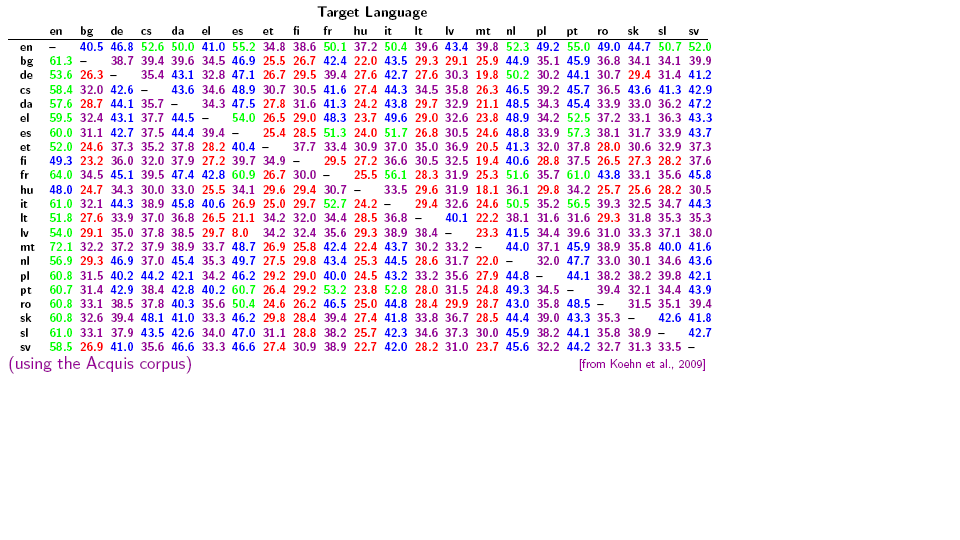
\includegraphics[scale=0.5]{media/grit.png}

	\subsection{Other Application Areas}
Building language technology applications involves a range of subtasks that do not always surface at the level of interaction with the user, but they provide significant service functionalities “under the hood” of the system in question. They all form important research issues that have now evolved into individual sub-disciplines of computational linguistics. 
Question answering, for example, is an active area of research for which annotated corpora have been built and scientific competitions have been initiated. The concept of question answering goes beyond keyword-based searches (in which the search engine responds by delivering a collection of potentially relevant documents) and enables users to ask a concrete question to which the system provides a single answer. For example: 
\begin{center}
\textit{Question: How old was Neil Armstrong when he stepped on the moon?\\
Answer: 38.}
\end{center}
While question answering is obviously related to the core area of web search, it is nowadays an umbrella term for such research issues as what different types of questions there are, and how they should be handled; how a set of documents that potentially contain the answer can be analysed and compared (do they provide conflicting answers?); and how specific information (the answer) can be reliably extracted from a document without ignoring the context. 
This is in turn related to information extraction (IE), an area that was extremely popular and influential when computational linguistics took a statistical turn in the early 1990s. IE aims to identify specific pieces of information in specific classes of documents, such as detecting the key players in company takeovers as reported in newspaper stories. Another common scenario that has been studied is reports on terrorist incidents. The problem here is to map the text to a template that specifies the perpetrator, target, time, location and results of the incident. Domain-specific template-filling is the central characteristic of IE, which makes it another example of a “behind the scenes” technology that forms a well-demarcated research area that in practice needs to be embedded into a suitable application environment. 
Text summarization and text generation are two borderline areas that can act either as standalone applications or play a supporting role “under the hood”. Summarization attempts to give the essentials of a long text in a short form, and is one of the features available in Microsoft Word. It mostly uses a statistical approach to identify the “important” words in a text (i.e., words that occur very frequently in the text in question but less frequently in general language use) and determine which sentences contain the most of these “important” words. These sentences are then extracted and put together to create the summary. In this very common commercial scenario, summarization is simply a form of sentence extraction, and the text is reduced to a subset of its sentences. An alternative approach, for which some research has been carried out, is to generate brand new sentences that do not exist in the source text. This requires a deeper understanding of the text, which means that so far this approach is far less robust. On the whole, a text generator is rarely used as a stand-alone application but is embedded into a larger software environment, such as a clinical information system that collects, stores and processes patient data. Creating reports is just one of many applications for text summarization. 
For the German language, research in these text technologies is much less developed than for the English language. Question answering, information extraction, and summarization have been the focus of numerous open competitions in the USA since the 1990s, primarily organised by the government-sponsored organisations DARPA and NIST. These competitions have significantly improved the start-of-the-art, but their focus has mostly been on the English language. As a result, there are hardly any annotated corpora or other special resources needed to perform these tasks in German. When summarization systems use purely statistical methods, they are largely language-independent and a number of research prototypes are available. For text generation, reusable components have traditionally been limited to surface realization modules (generation grammars) and most of the available software is for the English language. There is, however, a semantics-based multilingual generator and a template-based generator for the German language, but they date back to the 1990s and have not been ported to today’s software environments.
	
	\subsection{Educational Programmes}
Language technology is a very interdisciplinary field that involves the combined expertise of linguists, computer scientists, mathematicians, philosophers, psycholinguists, and neuroscientists among others. As a result, it has not acquired a clear, independent existence in the German faculty system. Some universities have established a separate institute for computational linguistics (CL) (e.g., Heidelberg, Saarbrücken and Tübingen); others have created institutes under a slightly different name (Stuttgart). Programmes are also offered by other departments, such as computer science faculties (Leipzig and Hamburg) or linguistics faculties (Bochum and Jena). Some universities only offer Master’s courses (Gießen) or Bachelor’s courses (Erlangen-Nürnberg, Göttingen, Munich, Potsdam and Trier), or language technology modules to students majoring in other subjects (Hildesheim). Many of these programmes and courses have only been introduced recently. At least 17 German universities currently offer programmes in the field of language technology. In Switzerland, CL programmes are offered by the Universities of Zurich and Geneva. In Austria, there is no fully-fledged CL study programme, but CL and LT courses are taught as part of other programmes in Vienna and Klagenfurt.
The German Federal Statistics Office has kept statistics on CL as a course of study at German universities since the Winter Semester of 1992-93. Since then, studying CL has become increasingly popular. The number of students has been stable since 2000, and programmes have annually attracted around 250-350 new students who enrol in CL as their main course of study.i This relatively low number of graduates from German universities cannot meet the steadily rising demand for qualified personnel specialized in language technology. In many cases, companies and research institutes such as the German Research Centre for Artificial Intelligence (DFKI) and the Austrian Research Institute for Artificial Intelligence (ÖFAI) have to call on foreign experts to help them with their work. 

	\subsection{National Projects and Efforts}
The existence of a relatively lively LT sector in Germany can be traced back to the major LT programmes over the last 20 to 30 years. One of the first was EUROTRA, an ambitious machine translation project that was established and funded by the European Commission from the late 1970s until 1994. Although EUROTRA did not manage to reach its stated goal of building a state-of-the-art translation system, the project did have a long-term impact on Europe’s language technology industry. The VERBMOBIL project focused on a more data-driven approach to LT following a major shift in the translation paradigm away from a rule-based approach. This large-scale national project with the goal of translating speech in real time between German, Japanese and English was funded by the Federal Ministry of Education and Research (BMBF) from 1993 to 2000. Although the resulting VERBMOBIL prototype was unable to establish itself in the marketplace, it lead to many spin-off innovations, and the technology now underlies the Google Translate system available on the Web. 
The IBM project LILOG, which ran from 1985 to 1991, was an implementation of an information base in the German language. It involved some 200 scientists working in computational linguistics, natural language understanding systems and artificial intelligence in Germany, and proved that a cooperative project between universities and industry can produce useful results for both pure research and real world methods and tools.
National projects focused on marking-up and annotating language resources were funded in the 1990s and early 2000. These led to the development of the Stuttgart-Tübingen tag set (STTS), which has had a lasting impact on the annotation of language corpora. Two other projects – NEGRA and TIGER – were partially funded by the German Research Foundation (DFG). The annotation schemes proposed by these projects have become the de facto standard in the field, and they now underlie the international standardisation of syntactic annotation.
COLLATE, funded by the BMBF from 2000 to 2006, was one of the first projects to address the issues of a language infrastructure and led to the creation of an information portal for the field (LT World). German and Austrian institutions are involved in the on-going European CLARIN project. Other on-going projects include EUROPEANA and THESEUS, a project co-funded by the Federal Ministry of Economics and Technology (BMWI) that aims to develop the basic technologies and standards needed to make knowledge on the Internet more widely available in the future. 
Along with many smaller scale projects that have now been completed, the above projects have led to the development of wide-ranging competence in the field of language technology as well as the creation of a basic technological infrastructure for German language tools and resources. Public funding for LT projects in Germany and in Europe is still relatively low, however, when compared to the amount of money the USA spends on language translation and multilingual information access.i 
In Austria, the Medical University of Vienna developed a language dialogue system in German as a part of the VIE-LANG project. The Faculty of Computer Sciences at the University of Vienna is carrying out the JETCAT project on translation between Japanese and English, and an on-going project has been compiling the Austrian Academy Corpus since 2001. There are no dedicated LT programmes in Austria. Funding for LT-related topics typically comes from research programmes that have open topics, especially those that focus on the transfer of knowledge from academic research to industry (particularly via SMEs). Several of these programmes are administered by the Austrian Research Promotion Agency (FFG). The Vienna Science and Technology Fund (WWTF) is a fairly strong supporter of localized language technology, especially for topics related to Vienna, such as synthesizing the speech of the Viennese dialect (or sociolect) and building MT systems to translate from Austrian German to Viennese and other dialects. 
In Switzerland, interest in language technology began in the 1980s with strong involvement in the EUROTRA project. The Universities of Zurich and Geneva are currently involved in several projects in the field of MT including MT between Standard German and Swiss German.ii Corpus-building projects include the collection of speech corpora by the National Centre of Competence in Research on Interactive Multimodal Information Management and a project that collects SMS text messages in Swiss German.iii Swiss research institutes in this field include ISSCO and IDIAP. Generally speaking, Switzerland has a small LT sector, mainly because of limited funding opportunities. EU funding is not always accessible and is often considered to be unattractive for Swiss SMEs. The Commission for Technology and Innovation (KTI) offers efficient, red-tape-free support for short and medium-term projects and also supports the development of start-up companies. However, start-ups in the field of language technology are rare due to this lack of relevant expertise.
As we have seen, previous programmes have led to the development of a number of LT tools and resources for the German language. In the following section, the current state of LT support for German is summarized.  

	\subsection{Availability of Tools and Resources}
The following table summarizes the current state of language technology support for the German language. The rating for existing tools and resources is based on estimates of leading experts.\\
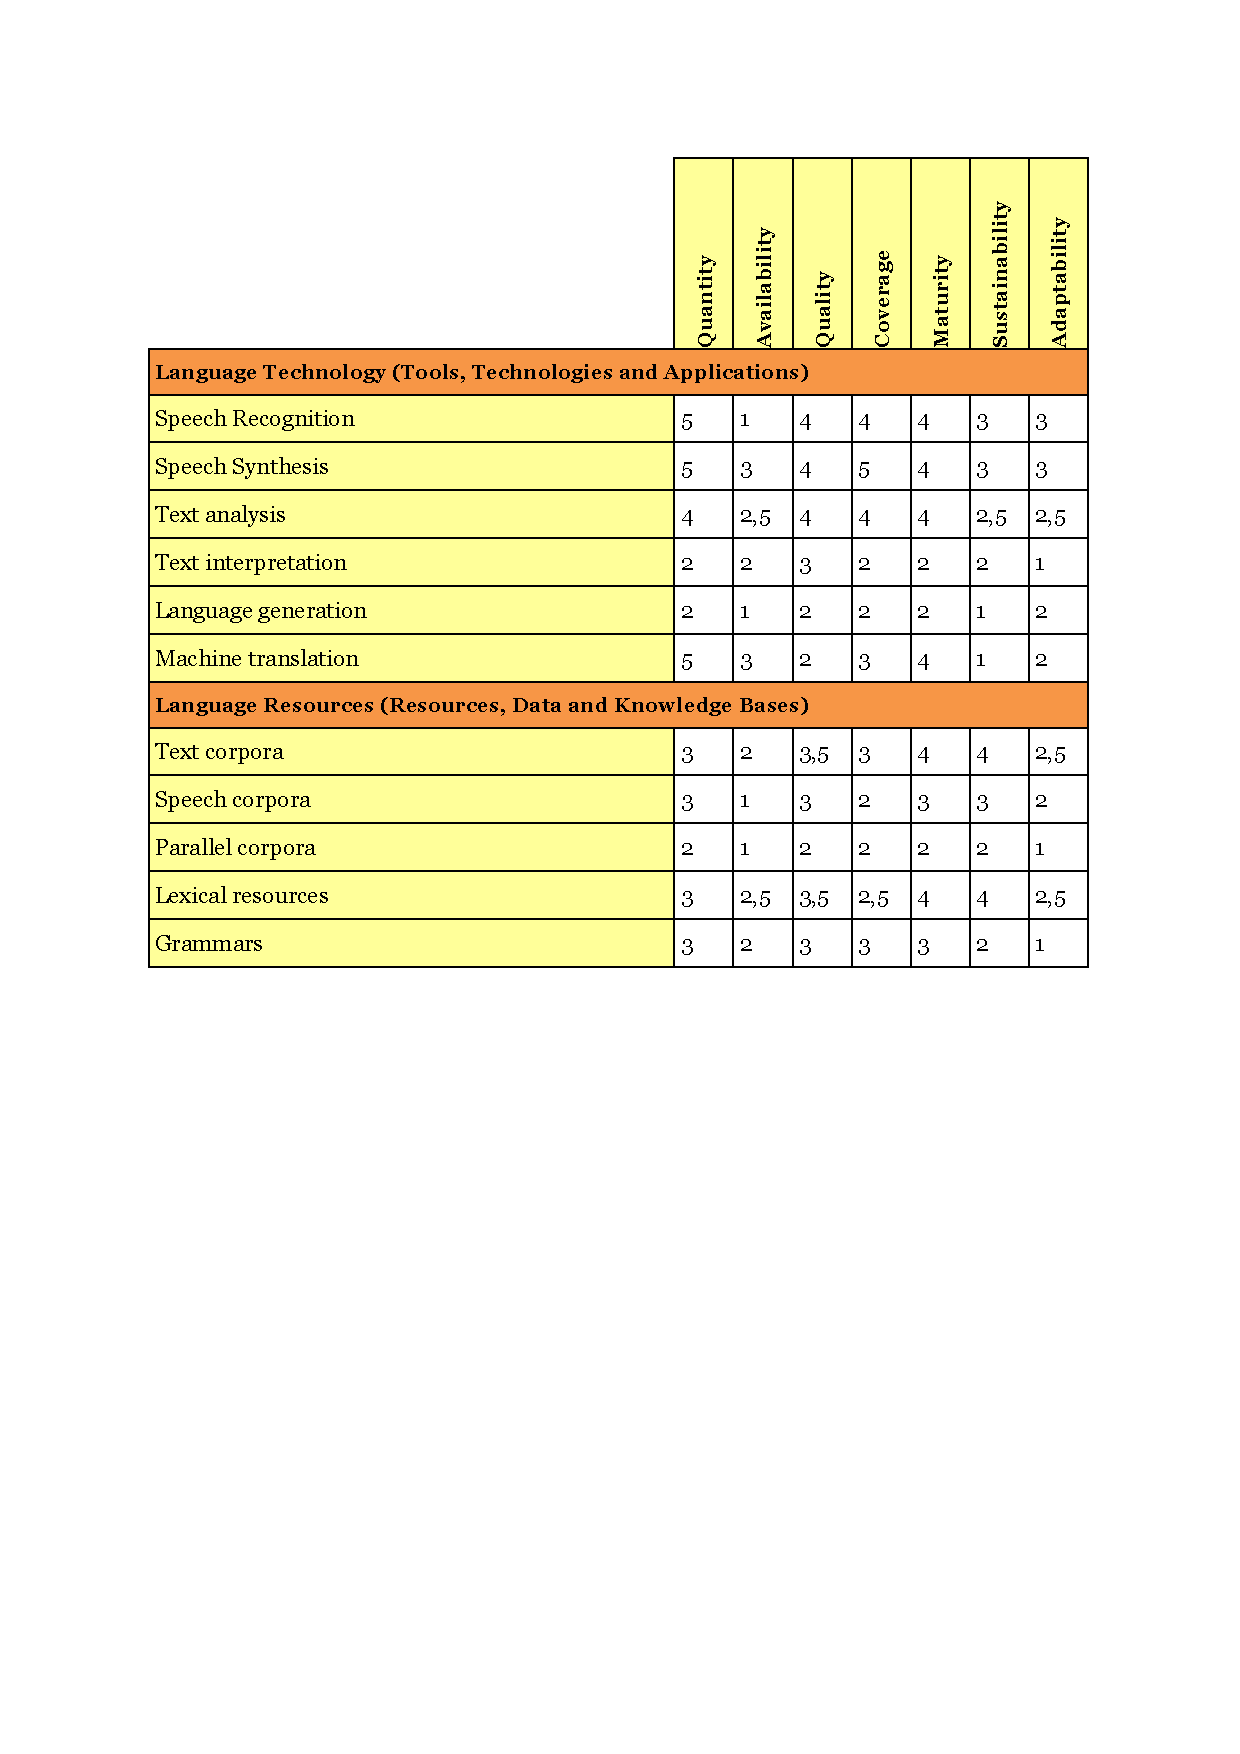
\includegraphics[scale=0.3]{media/metanet-paper2.pdf} 
The key results for the German language can be summed up as follows:
\begin{itemize}
\item Speech processing currently seems to be more mature than the processing of written text. In fact, speech technology has already been successfully integrated in many everyday applications, such as spoken dialogue systems and voice-based interfaces to mobile phones and car navigation systems.  
\item Research has been successful in designing medium to high quality software for basic text analysis, such as tools for morphological analysis and syntactic parsing, but advanced technologies that require deep linguistic processing and semantic knowledge are still in their infancy. 
\item As to resources, a large reference text corpus with a balanced mix of various genres for the German language exists, but access to it is difficult and expensive. There are some annotated corpora with syntactic, semantic and discourse structure mark-up, but again, the situation gets worse as the need for more deep linguistic and semantic information grows. 
\item In particular, there is a lack of parallel corpora, which form the basis of statistical and hybrid approaches to machine translation. Currently, translation from German to English works best because for this language pair large amounts of parallel texts are available. 
\item Many of the tools, resources and data formats are not standardised and cannot be sustained effectively. A concerted programme is required to standardise data formats and APIs.
\end{itemize}
For the German language we can conclude that for some specific areas, software with still limited functionality is available today. Obviously, further research efforts are required in order to meet current deficits for processing texts on a deeper semantic level and to address the lack of essential resources such as parallel corpora for machine translation. 

	\subsection{Cross-language comparison}
The current state of LT support varies considerably from one language to another. For comparing the situation across languages, this section will present an evaluation based on two sample application areas (machine translation and speech), one underlying technology (text analysis), as well as basic resources needed for building LT applications.\\ 
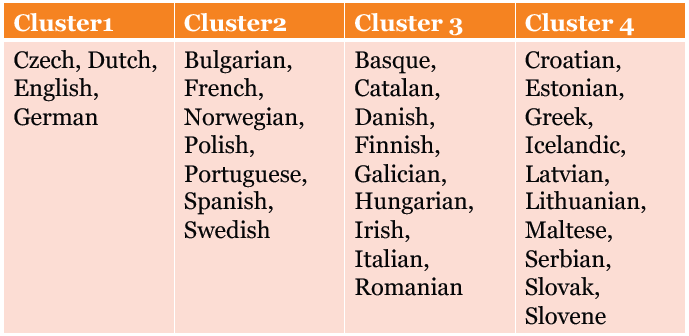
\includegraphics[scale=0.3]{media/bild.png}
The above tables show that, thanks to large-scale LT funding in the last decades, German is better equipped than most other languages. It compares well with languages with a similar number of speakers, such as French, despite its larger complexity. But LT resources and tools for German clearly do not yet reach the quality and coverage of comparable resources and tools for the English language, which takes the leading role in almost all areas. But even for the English language there are severe deficits with regard to high quality applications and resources.
For speech, currently available technologies perform well enough to be successfully integrated into a number of industrial applications such as spoken dialogue or dictation systems. Today’s text analysis components and language resources already cover the linguistic phenomena of German to a certain extent and are part of many applications involving mostly shallow natural language processing, e.g., spelling correction and authoring support.
However, for building more sophisticated applications, such as machine translation, there is an obvious lack of resources and technologies that cover a wider range of linguistic aspects and allow a deep, semantic analysis of the input text. Improving the quality and coverage of these basic resources and technologies will open up the opportunity to a vast range of advanced application areas, including high-quality machine translation that can be used in a variety of applications. 

	\subsection{Conclusions}
In this series of white papers, an important initial effort has been made to assess language technology support for 30 European languages and to compare the situation across languages at a high-level. Based on the identified gaps, needs and deficits the European language technology community and related stakeholders are now able to design a large scale research and development programme towards a technology enabled truly multilingual Europe.
Comparing the situation across languages, we have seen that the differences are immense. While for some languages and application areas, good quality software and resources are already available, substantial gaps have appeared for other languages, in particular small languages. Many languages lack already basic technologies for text analysis and essential resources needed for developing these technologies. For others, basic tools and resources are available but semantic processing is not possible. For all languages, there are still large efforts needed in order to reach ambitious goals such as high-quality machine translation for all European languages.  
As to the German language, we can be cautiously optimistic about the current state of language technology support. There is a viable LT research community in Germany, Austria and Switzerland, which have in the past been supported by large research programmes, many of them carried out in cooperation with industrial players such as Philips and IBM. A number of large-scale resources and state-of-the-art technologies have been produced and distributed for Standard German. However, the size of the resources and the number of tools is still very limited when compared to the resources and tools for the English language, and they are simply not ready to develop the technologies required to support a truly multilingual knowledge society.
Technologies that were developed and optimised for the English language do not easily transfer to German. For example identical systems for parsing (syntactic and grammatical analysis of sentence structure) typically perform far less well on German texts. This is due to the specific characteristics of the German language, such as free word order or long, nested sentences that require more sophisticated processing.
To date, there is a scattered and heterogeneous language technology industry at work on the German language. Most large companies have stopped or severely reduced their LT efforts, leaving the field to a number of specialized SMEs that are unable to address the internal and the global market. 
Our findings show that greater efforts to create LT resources for German, and drive research, innovation and development in general are inevitable. The need for large amounts of data and the extreme complexity of language technology systems makes it vital to develop a new infrastructure and improved research organization to spur greater sharing and cooperation.
There is a lack of continuity in research and development funding. Short-term coordinated programmes tend to alternate with periods of sparse funding or no funding at all. In addition, there is an overall lack of coordination among programmes in other EU countries and at the European Commission level.
On the basis of the insights gained so far, a large coordinated effort covering the whole of Europe focused on language technologies is desperately needed.
Modern language technology based on hybrid methods will enable the goal of bridging the gap between all European languages and beyond. As this white paper series shows, the difference in readiness of solutions and the state of research for the different languages is dramatic. 
The long-term perspective of META-NET is that high-quality language technology, which is available for all languages, will perfect the political and economic unity in cultural diversity, where language barriers are torn down and bridges are built between Europe’s languages. This requires a united effort of all stakeholders from politics, research, economy, and society.

	\section{About META-NET}
META-NET is a Network of Excellence funded by the European Commission. The network currently consists of 47 members from 31 European countries. META-NET fosters the Multilingual Europe Technology Alliance (META), a growing community of language technology professionals and organisations in Europe. 
META-NET cooperates with other initiatives like the Common Language Resources and Technology Infrastructure (CLARIN), which is helping establish digital humanities research in Europe. META-NET fosters the technological foundations for a truly multilingual European information society that:
\begin{itemize}
\item makes communication and cooperation possible across languages;
\item provides equal access to information and knowledge in any language;
\item offers advanced and affordable networked information technology to European citizens.
\end{itemize}
META-NET stimulates and promotes multilingual technologies for all European languages. The technologies enable automatic translation, content production, information processing and knowledge management for a wide variety of applications and subject domains. The network wants to improve current approaches, so better communication and cooperation across languages can take place. Europeans have an equal right to information and knowledge regardless of language. 
 
 	\subsection{Lines of Action}
 META-NET launched on 1 February 2010 with the goal of advancing research in language technology (LT). The network supports a Europe that unites as a single digital market and information space. META-NET has conducted several activities that further its goals. META-VISION, META-SHARE and META-RESEARCH are the network’s three lines of action.

Three Lines of Action in META-NET
META-VISION fosters a dynamic and influential stakeholder community that unites around a shared vision and a common strategic research agenda (SRA). The main focus of this activity is to build a coherent and cohesive LT community in Europe by bringing together representatives from highly fragmented and diverse groups of stakeholders. In the first year of META-NET, presentations at the FLaReNet Forum (Spain), Language Technology Days (Luxembourg), JIAMCATT 2010 (Luxembourg), LREC 2010 (Malta), EAMT 2010 (France) and ICT 2010 (Belgium) centred on public outreach. According to initial estimates, META-NET has already contacted more than 2,500 LT professionals to develop its goals and visions with them. At the META-FORUM 2010 event in Brussels, META-NET communicated the initial results of its vision building process to more than 250 participants. In a series of interactive sessions, the participants provided feedback on the visions presented by the network. 
META-SHARE creates an open, distributed facility for exchanging and sharing resources. The peer-to-peer network of repositories will contain language data, tools and web services that are documented with high-quality metadata and organised in standardised categories. The resources can be readily accessed and uniformly searched. The available resources include free, open source materials as well as restricted, commercially available, fee-based items. META-SHARE targets existing language data, tools and systems as well as new and emerging products that are required for building and evaluating new technologies, products and services. The reuse, combination, repurposing and re-engineering of language data and tools plays a crucial role. META-SHARE will eventually become a critical part of the LT marketplace for developers, localisation experts, researchers, translators and language professionals from small, mid-sized and large enterprises. META-SHARE addresses the full development cycle of LT—from research to innovative products and services. A key aspect of this activity is establishing META-SHARE as an important and valuable part of a European and global infrastructure for the LT community. 
META-RESEARCH builds bridges to related technology fields. This activity seeks to leverage advances in other fields and to capitalise on innovative research that can benefit language technology. In particular, this activity wants to bring more semantics into machine translation (MT), optimise the division of labour in hybrid MT, exploit context when computing automatic translations and prepare an empirical base for MT. META-RESEARCH is working with other fields and disciplines, such as machine learning and the Semantic Web community. META-RESEARCH focuses on collecting data, preparing data sets and organising language resources for evaluation purposes; compiling inventories of tools and methods; and organising workshops and training events for members of the community. This activity has already clearly identified aspects of MT where semantics can impact current best practices. In addition, the activity has created recommendations on how to approach the problem of integrating semantic information in MT. META-RESEARCH is also finalising a new language resource for MT, the Annotated Hybrid Sample MT Corpus, which provides data for English-German, English-Spanish and English-Czech language pairs. META-RESEARCH has also developed software that collects multilingual corpora that are hidden on the Web.

	\subsection{Member Organisations}

\begin{tabular}{|p{1.5cm}|p{3cm}|p{5cm}|}
\hline Country & Organisation & Participant(s) \\ 
\hline Austria & University of Vienna & Gerhard Budin\\
\hline Belgium & University of Antwerp & Walter Daelemans\\
\hline University of Leuven & Dirk van Compernolle & \\
\hline Bulgaria & Bulgarian Academy of Sciences & Svetla Koeva \\
\hline Croatia & University of Zagreb & Marko Tadić\\
\hline Cyprus & University of Cyprus & Jack Burston\\
\hline Czech Republic & Charles University in Prague Jan Hajic\\
\hline Denmark & University of Copenhagen & Bolette Sandford Pedersen and
Bente Maegaard\\
\hline Estonia & University of Tartu & Tiit Roosmaa\\
\hline Finland & Aalto University & Timo Honkela\\
\hline  & University of Helsinki & Kimmo Koskenniemi and
Krister Linden \\
\hline France & CNRS/LIMSI & Joseph Mariani \\
\hline & Evaluations and Language Resources Distribution Agency & Khalid Choukri\\
\hline Germany & DFKI & Hans Uszkoreit and Georg Rehm\\
\hline & RWTH Aachen University & Hermann Ney\\
\hline & Saarland University & Manfred Pinkal\\
\hline Greece & Institute for Language and Speech Processing, “Athena” R.C. & Stelios Piperidis\\
\hline Hungary & Hungarian Academy of Sciences & Tamás Váradi\\
\hline & Budapest University of Technology and Economics & Géza Németh and Gábor Olaszy\\
\hline Iceland & University of Iceland & Eirikur Rögnvaldsson\\
\end{tabular}
	%\clearpage
	
\begin{tabular}{|p{1.5cm}|p{3cm}|p{5cm}|}	
\hline Ireland & Dublin City University & Josef van Genabith\\
\hline Italy & Consiglio Nazionale Ricerche,  Istituto di Linguistica Computazionale “Antonio Zampolli” & Nicoletta Calzolari\\
\hline & Fondazione Bruno Kessler & Bernardo Magnini\\
\hline Latvia & Tilde & Andrejs Vasiljevs\\
\hline & Institute of Mathematics and Computer Science, University of Latvia & Inguna Skadina\\
\hline Lithuania & Institute of the Lithuanian Language & Jolanta Zabarskaitė\\
\hline Luxembourg & Arax Ltd. & Vartkes Goetcherian\\
\hline Malta & University of Malta & Mike Rosner\\
\hline Netherlands & Utrecht University & Jan Odijk\\
\hline & University of Groningen & Gertjan van Noord\\
\hline Norway & University of Bergen & Koenraad De Smedt\\
\hline Poland & Polish Academy of Sciences & Adam Przepiórkowski and
Maciej Ogrodniczuk \\
\hline & University of Lodz & Barbara Lewandowska-Tomaszczyk and Piotr Pęzik\\
\hline Portugal & University of Lisbon & Antonio Branco\\
\hline & Institute for Systems Engineering and Computers & Isabel Trancoso\\
\hline Romania & Romanian Academy of Sciences & Dan Tufis\\
\hline & Alexandru Ioan Cuza University & Dan Cristea\\
\hline Serbia & University of Belgrade & Dusko Vitas, Cvetana Krstev and
Ivan Obradovic\\
\hline & Institute Mihailo Pupin & Sanja Vranes\\
\hline Slovakia & Slovak Academy of Sciences & Radovan Garabik\\
\end{tabular}

\begin{tabular}{|p{1.5cm}|p{3cm}|p{5cm}|}
\hline Slovenia & Jozef Stefan Institute & Marko Grobelnik\\
\hline Spain & Barcelona Media & Toni Badia\\
\hline & Technical University of Catalonia & Asunción Moreno\\
\hline  & Pompeu Fabra University & Núria Bel\\
\hline Sweden & University of Gothenburg & Lars Borin\\
\hline UK & University of Manchester & Sophia Ananiadou\\
\hline & University of Edinburgh & Steve Renals\\
\hline  & & \\
\end{tabular}  
	
 \subsection{References}
 European Commission, Multilingualism: an asset for Europe and a shared commitment, Brussels, 2008 (http://ec.europa.eu/education/languages/pdf/com/2008\_0566\_en.pdf).\\
  UNESCO Director-General, Intersectoral mid-term strategy on languages and multilingualism, Paris, 2007 (http://unesdoc.unesco.org/images/0015/001503/150335e.pdf).\\
  European Commission Directorate-General for Translation, Size of the language industry in the EU, Kingston Upon Thames, 2009 (http://ec.europa.eu/dgs/translation/publications/studies).\\
   http://cdt.europa.eu/EN/whoweare/Pages/OurEUlanguages.aspx\\
    http://www.goethe.de/mmo/priv/1459127-STANDARD.pdf\\
 http://www.efnil.org/documents/language-legislation-version-2007/germany/germany\\
  http://www.canoo.net/services/GermanSpelling/Reform/fremdwoerter/eindeutschung-lebend.jsp?MenuId=GermanSpellingReform111\\ Lothar Lemnitzer: Von Aldianer bis Zauselquote, Gunter Narr Verlag Tübingen, 2007.\\
 Bastian Sick: Der Dativ ist dem Genitiv sein Tod – Ein Wegweiser durch den Irrgarten der deutschen Sprache, Kiepenheuer und Witsch, Köln, 2004. \\
 http://www.spiegel.de/thema/zwiebelfisch/\\
 Wolf Schneider: Speak German! – Warum Deutsch manchmal besser ist. Rowohlt, 2008.\\
 “PISA 2009 Ergebnisse: Zusammenfassung”,  http://www.pisa.oecd.org/dataoecd/34/19/46619755.pdf\\
 http://www.kmk.org/fileadmin/veroeffentlichungen\_beschluesse/2003/2003\_01\_01-Bildungsbericht-erste-Befunde.pdf\\
 http://userweb.port.ac.uk/\textasciitilde joyce1/abinitio/whygerm7.html\\
 http://www.ard-zdf-onlinestudie.de and \\ http://www.statistik.at/web\_en/statistics/information\_society/ict\_usage\_in\_households/041019.html\\
 http://www.denic.de/hintergrund/geschichte-der-denic-eg.html and http://www.ebrandservices.com/welcome-to-e-brand-services,130.html\\
 http://dict.leo.org/\\
 Jerrold H. Zar: “Candidate for a Pullet Surprise”, Journal of Irreproducible Results, Jan/Feb. 1994, page 13 (first verse). \\
 Anne Lehrndorferand Stefanie Schachtl: “TR09: Controlled Siemens Documentary German and TopTrans”, TC Forum, 1998.\\
 http://www.spiegel.de/netzwelt/web/0,1518,619398,00.html\\
 http://www.pcworld.com/businesscenter/article/161869/google\_rolls\_out\_semantic\_search\_capabilities.html\\
 K. Papineni, S. Roukos, T. Ward, W.-J. Zhu. BLEU: A Method for Automatic Evaluation of Machine Translation. In Proceedings of the 40th Annual Meeting of ACL, Philadelphia, PA.\\
 Based on official university statistics of the Federal Statistical Office in  Wiesbaden (29.03.2011)\\
 Gianni Lazzari: “Sprachtechnologien für Europa”, 2006:  http://tcstar.org/pubblicazioni/D17\_HLT\_DE.pdf \\
 http://www.latl.unige.ch/personal/yvesscherrer/\#talks\_papers.fr \\
  Claudia Soria, Joseph Mariani(2011): “Report on Existing Projects and Initiatives” and http://www.sms4science.ch/\\

\section{LOREM ISPUM}
\subsection{IPSUM LOREM}
Lorem ipsum dolor sit amet, consetetur sadipscing elitr, sed diam nonumy eirmod tempor invidunt ut labore et dolore magna aliquyam erat, sed diam voluptua. At vero eos et accusam et justo duo dolores et ea rebum. Stet clita kasd gubergren, no sea takimata sanctus est Lorem ipsum dolor sit amet. Lorem ipsum dolor sit amet, consetetur sadipscing elitr, sed diam nonumy eirmod tempor invidunt ut labore et dolore magna aliquyam erat, sed diam voluptua. At vero eos et accusam et justo duo dolores et ea rebum. Stet clita kasd gubergren, no sea takimata sanctus est Lorem ipsum dolor sit amet. Lorem ipsum dolor sit amet, consetetur sadipscing elitr, sed diam nonumy eirmod tempor invidunt ut labore et dolore magna aliquyam erat, sed diam voluptua. At vero eos et accusam et justo duo dolores et ea rebum. Stet clita kasd gubergren, no sea takimata sanctus est Lorem ipsum dolor sit amet.   

Duis autem vel eum iriure dolor in hendrerit in vulputate velit esse molestie consequat, vel illum dolore eu feugiat nulla facilisis at vero eros et accumsan et iusto odio dignissim qui blandit praesent luptatum zzril delenit augue duis dolore te feugait nulla facilisi. Lorem ipsum dolor sit amet, consectetuer adipiscing elit, sed diam nonummy nibh euismod tincidunt ut laoreet dolore magna aliquam erat volutpat.   

Ut wisi enim ad minim veniam, quis nostrud exerci tation ullamcorper suscipit lobortis nisl ut aliquip ex ea commodo consequat. Duis autem vel eum iriure dolor in hendrerit in vulputate velit esse molestie consequat, vel illum dolore eu feugiat nulla facilisis at vero eros et accumsan et iusto odio dignissim qui blandit praesent luptatum zzril delenit augue duis dolore te feugait nulla facilisi.   

Nam liber tempor cum soluta nobis eleifend option congue nihil imperdiet doming id quod mazim placerat facer possim assum. Lorem ipsum dolor sit amet, consectetuer adipiscing elit, sed diam nonummy nibh euismod tincidunt ut laoreet dolore magna aliquam erat volutpat. Ut wisi enim ad minim veniam, quis nostrud exerci tation ullamcorper suscipit lobortis nisl ut aliquip ex ea commodo consequat.   
\subsection{IPSUM LOREM}
Duis autem vel eum iriure dolor in hendrerit in vulputate velit esse molestie consequat, vel illum dolore eu feugiat nulla facilisis.   

At vero eos et accusam et justo duo dolores et ea rebum. Stet clita kasd gubergren, no sea takimata sanctus est Lorem ipsum dolor sit amet. Lorem ipsum dolor sit amet, consetetur sadipscing elitr, sed diam nonumy eirmod tempor invidunt ut labore et dolore magna aliquyam erat, sed diam voluptua. At vero eos et accusam et justo duo dolores et ea rebum. Stet clita kasd gubergren, no sea takimata sanctus est Lorem ipsum dolor sit amet. Lorem ipsum dolor sit amet, consetetur sadipscing elitr, At accusam aliquyam diam diam dolore dolores duo eirmod eos erat, et nonumy sed tempor et et invidunt justo labore Stet clita ea et gubergren, kasd magna no rebum. sanctus sea sed takimata ut vero voluptua. est Lorem ipsum dolor sit amet. Lorem ipsum dolor sit amet, consetetur sadipscing elitr, sed diam nonumy eirmod tempor invidunt ut labore et dolore magna aliquyam erat.   

Consetetur sadipscing elitr, sed diam nonumy eirmod tempor invidunt ut labore et dolore magna aliquyam erat, sed diam voluptua. At vero eos et accusam et justo duo dolores et ea rebum. Stet clita kasd gubergren, no sea takimata sanctus est Lorem ipsum dolor sit amet. Lorem ipsum dolor sit amet, consetetur sadipscing elitr, sed diam nonumy eirmod tempor invidunt ut labore et dolore magna aliquyam erat, sed diam voluptua. At vero eos et accusam et justo duo dolores et ea rebum. Stet clita kasd gubergren, no sea takimata sanctus est Lorem ipsum dolor sit amet. Lorem ipsum dolor sit amet, consetetur sadipscing elitr, sed diam nonumy eirmod tempor invidunt ut labore et dolore magna aliquyam erat, sed diam voluptua. At vero eos et accusam et justo duo dolores et ea rebum. Stet clita kasd gubergren, no sea takimata sanctus.   
\section{LOREM ISPUM}
Lorem ipsum dolor sit amet, consetetur sadipscing elitr, sed diam nonumy eirmod tempor invidunt ut labore et dolore magna aliquyam erat, sed diam voluptua. At vero eos et accusam et justo duo dolores et ea rebum. Stet clita kasd gubergren, no sea takimata sanctus est Lorem ipsum dolor sit amet. Lorem ipsum dolor sit amet, consetetur sadipscing elitr, sed diam nonumy eirmod tempor invidunt ut labore et dolore magna aliquyam erat, sed diam voluptua. At vero eos et accusam et justo duo dolores et ea rebum. Stet clita kasd gubergren, no sea takimata sanctus est Lorem ipsum dolor sit amet. Lorem ipsum dolor sit amet, consetetur sadipscing elitr, sed diam nonumy eirmod tempor invidunt ut labore et dolore magna aliquyam erat, sed diam voluptua. At vero eos et accusam et justo duo dolores et ea rebum. Stet clita kasd gubergren, no sea takimata sanctus est Lorem ipsum dolor sit amet.   

Duis autem vel eum iriure dolor in hendrerit in vulputate velit esse molestie consequat, vel illum dolore eu feugiat nulla facilisis at vero eros et accumsan et iusto odio dignissim qui blandit praesent luptatum zzril delenit augue duis dolore te feugait nulla facilisi. Lorem ipsum dolor sit amet, consectetuer adipiscing elit, sed diam nonummy nibh euismod tincidunt ut laoreet dolore magna aliquam erat volutpat.   

Ut wisi enim ad minim veniam, quis nostrud exerci tation ullamcorper suscipit lobortis nisl ut aliquip ex ea commodo consequat. Duis autem vel eum iriure dolor in hendrerit in vulputate velit esse molestie consequat, vel illum dolore eu feugiat nulla facilisis at vero eros et accumsan et iusto odio dignissim qui blandit praesent luptatum zzril delenit augue duis dolore te feugait nulla facilisi.   

Nam liber tempor cum soluta nobis eleifend option congue nihil imperdiet doming id quod mazim placerat facer possim assum. Lorem ipsum dolor sit amet, consectetuer adipiscing elit, sed diam nonummy nibh euismod tincidunt ut laoreet dolore magna aliquam erat volutpat. Ut wisi enim ad minim veniam, quis nostrud exerci tation ullamcorper suscipit lobortis nisl ut aliquip ex ea commodo consequat.   

Duis autem vel eum iriure dolor in hendrerit in vulputate velit esse molestie consequat, vel illum dolore eu feugiat nulla facilisis.   

At vero eos et accusam et justo duo dolores et ea rebum. Stet clita kasd gubergren, no sea takimata sanctus est Lorem ipsum dolor sit amet. Lorem ipsum dolor sit amet, consetetur sadipscing elitr, sed diam nonumy eirmod tempor invidunt ut labore et dolore magna aliquyam erat, sed diam voluptua. At vero eos et accusam et justo duo dolores et ea rebum. Stet clita kasd gubergren, no sea takimata sanctus est Lorem ipsum dolor sit amet. Lorem ipsum dolor sit amet, consetetur sadipscing elitr, At accusam aliquyam diam diam dolore dolores duo eirmod eos erat, et nonumy sed tempor et et invidunt justo labore Stet clita ea et gubergren, kasd magna no rebum. sanctus sea sed takimata ut vero voluptua. est Lorem ipsum dolor sit amet. Lorem ipsum dolor sit amet, consetetur sadipscing elitr, sed diam nonumy eirmod tempor invidunt ut labore et dolore magna aliquyam erat.   

Consetetur sadipscing elitr, sed diam nonumy eirmod tempor invidunt ut labore et dolore magna aliquyam erat, sed diam voluptua. At vero eos et accusam et justo duo dolores et ea rebum. Stet clita kasd gubergren, no sea takimata sanctus est Lorem ipsum dolor sit amet. Lorem ipsum dolor sit amet, consetetur sadipscing elitr, sed diam nonumy eirmod tempor invidunt ut labore et dolore magna aliquyam erat, sed diam voluptua. At vero eos et accusam et justo duo dolores et ea rebum. Stet clita kasd gubergren, no sea takimata sanctus est Lorem ipsum dolor sit amet. Lorem ipsum dolor sit amet, consetetur sadipscing elitr, sed diam nonumy eirmod tempor invidunt ut labore et dolore magna aliquyam erat, sed diam voluptua. At vero eos et accusam et justo duo dolores et ea rebum. Stet clita kasd gubergren, no sea takimata sanctus.   

Lorem ipsum dolor sit amet, consetetur sadipscing elitr, sed diam nonumy eirmod tempor invidunt ut labore et dolore magna aliquyam erat, sed diam voluptua. At vero eos et accusam et justo duo dolores et ea rebum. Stet clita kasd gubergren, no sea takimata sanctus est Lorem ipsum dolor sit amet. Lorem ipsum dolor sit amet, consetetur sadipscing elitr, sed diam nonumy eirmod tempor invidunt ut labore et dolore magna aliquyam erat, sed diam voluptua. At vero eos et accusam et justo duo dolores et ea rebum. Stet clita kasd gubergren, no sea takimata sanctus est Lorem ipsum dolor sit amet. Lorem ipsum dolor sit amet, consetetur sadipscing elitr, sed diam nonumy eirmod tempor invidunt ut labore et dolore magna aliquyam erat, sed diam voluptua. At vero eos et accusam et justo duo dolores et ea rebum. Stet clita kasd gubergren, no sea takimata sanctus est Lorem ipsum dolor sit amet.   

Duis autem vel eum iriure dolor in hendrerit in vulputate velit esse molestie consequat, vel illum dolore eu feugiat nulla facilisis at vero eros et accumsan et iusto odio dignissim qui blandit praesent luptatum zzril delenit augue duis dolore te feugait nulla facilisi. Lorem ipsum dolor sit amet, consectetuer adipiscing elit, sed diam nonummy nibh euismod tincidunt ut laoreet dolore magna aliquam erat volutpat.   

Ut wisi enim ad minim veniam, quis nostrud exerci tation ullamcorper suscipit lobortis nisl ut aliquip ex ea commodo consequat. Duis autem vel eum iriure dolor in hendrerit in vulputate velit esse molestie consequat, vel illum dolore eu feugiat nulla facilisis at vero eros et accumsan et iusto odio dignissim qui blandit praesent luptatum zzril delenit augue duis dolore te feugait nulla facilisi.   

Nam liber tempor cum soluta nobis eleifend option congue nihil imperdiet doming id quod mazim placerat facer possim assum. Lorem ipsum dolor sit amet, consectetuer adipiscing elit, sed diam nonummy nibh euismod tincidunt ut laoreet dolore magna aliquam erat volutpat. Ut wisi enim ad minim veniam, quis nostrud exerci tation ullamcorper suscipit lobortis nisl ut aliquip ex ea commodo consequat.   
\subsection{IPSUM LOREM}
Duis autem vel eum iriure dolor in hendrerit in vulputate velit esse molestie consequat, vel illum dolore eu feugiat nulla facilisis.   

At vero eos et accusam et justo duo dolores et ea rebum. Stet clita kasd gubergren, no sea takimata sanctus est Lorem ipsum dolor sit amet. Lorem ipsum dolor sit amet, consetetur sadipscing elitr, sed diam nonumy eirmod tempor invidunt ut labore et dolore magna aliquyam erat, sed diam voluptua. At vero eos et accusam et justo duo dolores et ea rebum. Stet clita kasd gubergren, no sea takimata sanctus est Lorem ipsum dolor sit amet. Lorem ipsum dolor sit amet, consetetur sadipscing elitr, At accusam aliquyam diam diam dolore dolores duo eirmod eos erat, et nonumy sed tempor et et invidunt justo labore Stet clita ea et gubergren, kasd magna no rebum. sanctus sea sed takimata ut vero voluptua. est Lorem ipsum dolor sit amet. Lorem ipsum dolor sit amet, consetetur sadipscing elitr, sed diam nonumy eirmod tempor invidunt ut labore et dolore magna aliquyam erat.   
\section{LOREM ISPUM}
Consetetur sadipscing elitr, sed diam nonumy eirmod tempor invidunt ut labore et dolore magna aliquyam erat, sed diam voluptua. At vero eos et accusam et justo duo dolores et ea rebum. Stet clita kasd gubergren, no sea takimata sanctus est Lorem ipsum dolor sit amet. Lorem ipsum dolor sit amet, consetetur sadipscing elitr, sed diam nonumy eirmod tempor invidunt ut labore et dolore magna aliquyam erat, sed diam voluptua. At vero eos et accusam et justo duo dolores et ea rebum. Stet clita kasd gubergren, no sea takimata sanctus est Lorem ipsum dolor sit amet. Lorem ipsum dolor sit amet, consetetur sadipscing elitr, sed diam nonumy eirmod tempor invidunt ut labore et dolore magna aliquyam erat, sed diam voluptua. At vero eos et accusam et justo duo dolores et ea rebum. Stet clita kasd gubergren, no sea takimata sanctus.   

Lorem ipsum dolor sit amet, consetetur sadipscing elitr, sed diam nonumy eirmod tempor invidunt ut labore et dolore magna aliquyam erat, sed diam voluptua. At vero eos et accusam et justo duo dolores et ea rebum. Stet clita kasd gubergren, no sea takimata sanctus est Lorem ipsum dolor sit amet. Lorem ipsum dolor sit amet, consetetur sadipscing elitr, sed diam nonumy eirmod tempor invidunt ut labore et dolore magna aliquyam erat, sed diam voluptua. At vero eos et accusam et justo duo dolores et ea rebum. Stet clita kasd gubergren, no sea takimata sanctus est Lorem ipsum dolor sit amet. Lorem ipsum dolor sit amet, consetetur sadipscing elitr, sed diam nonumy eirmod tempor invidunt ut labore et dolore magna aliquyam erat, sed diam voluptua. At vero eos et accusam et justo duo dolores et ea rebum. Stet clita kasd gubergren, no sea takimata sanctus est Lorem ipsum dolor sit amet.   

Duis autem vel eum iriure dolor in hendrerit in vulputate velit esse molestie consequat, vel illum dolore eu feugiat nulla facilisis at vero eros et accumsan et iusto odio dignissim qui blandit praesent luptatum zzril delenit augue duis dolore te feugait nulla facilisi. Lorem ipsum dolor sit amet, consectetuer adipiscing elit, sed diam nonummy nibh euismod tincidunt ut laoreet dolore magna aliquam erat volutpat.   

Ut wisi enim ad minim veniam, quis nostrud exerci tation ullamcorper suscipit lobortis nisl ut aliquip ex ea commodo consequat. Duis autem vel eum iriure dolor in hendrerit in vulputate velit esse molestie consequat, vel illum dolore eu feugiat nulla facilisis at vero eros et accumsan et iusto odio dignissim qui blandit praesent luptatum zzril delenit augue duis dolore te feugait nulla facilisi.   

Nam liber tempor cum soluta nobis eleifend option congue nihil imperdiet doming id quod mazim placerat facer possim assum. Lorem ipsum dolor sit amet, consectetuer adipiscing elit, sed diam nonummy nibh euismod tincidunt ut laoreet dolore magna aliquam erat volutpat. Ut wisi enim ad minim veniam, quis nostrud exerci tation ullamcorper suscipit lobortis nisl ut aliquip ex ea commodo consequat.   

Duis autem vel eum iriure dolor in hendrerit in vulputate velit esse molestie consequat, vel illum dolore eu feugiat nulla facilisis.   

At vero eos et accusam et justo duo dolores et ea rebum. Stet clita kasd gubergren, no sea takimata sanctus est Lorem ipsum dolor sit amet. Lorem ipsum dolor sit amet, consetetur sadipscing elitr, sed diam nonumy eirmod tempor invidunt ut labore et dolore magna aliquyam erat, sed diam voluptua. At vero eos et accusam et justo duo dolores et ea rebum. Stet clita kasd gubergren, no sea takimata sanctus est Lorem ipsum dolor sit amet. Lorem ipsum dolor sit amet, consetetur sadipscing elitr, At accusam aliquyam diam diam dolore dolores duo eirmod eos erat, et nonumy sed tempor et et invidunt justo labore Stet clita ea et gubergren, kasd magna no rebum. sanctus sea sed takimata ut vero voluptua. est Lorem ipsum dolor sit amet. Lorem ipsum dolor sit amet, consetetur sadipscing elitr, sed diam nonumy eirmod tempor invidunt ut labore et dolore magna aliquyam erat.   

Consetetur sadipscing elitr, sed diam nonumy eirmod tempor invidunt ut labore et dolore magna aliquyam erat, sed diam voluptua. At vero eos et accusam et justo duo dolores et ea rebum. Stet clita kasd gubergren, no sea takimata sanctus est Lorem ipsum dolor sit amet. Lorem ipsum dolor sit amet, consetetur sadipscing elitr, sed diam nonumy eirmod tempor invidunt ut labore et dolore magna aliquyam erat, sed diam voluptua. At vero eos et accusam et justo duo dolores et ea rebum. Stet clita kasd gubergren, no sea takimata sanctus est Lorem ipsum dolor sit amet. Lorem ipsum dolor sit amet, consetetur sadipscing elitr, sed diam nonumy eirmod tempor invidunt ut labore et dolore magna aliquyam erat, sed diam voluptua. At vero eos et accusam et justo duo dolores et ea rebum. Stet clita kasd gubergren, no sea takimata sanctus.   

Lorem ipsum dolor sit amet, consetetur sadipscing elitr, sed diam nonumy eirmod tempor invidunt ut labore et dolore magna aliquyam erat, sed diam voluptua. At vero eos et accusam et justo duo dolores et ea rebum. Stet clita kasd gubergren, no sea takimata sanctus est Lorem ipsum dolor sit amet. Lorem ipsum dolor sit amet, consetetur sadipscing elitr, sed diam nonumy eirmod tempor invidunt ut labore et dolore magna aliquyam erat, sed diam voluptua. At vero eos et accusam et justo duo dolores et ea rebum. Stet clita kasd gubergren, no sea takimata sanctus est Lorem ipsum dolor sit amet. Lorem ipsum dolor sit amet, consetetur sadipscing elitr, sed diam nonumy eirmod tempor invidunt ut labore et dolore magna aliquyam erat, sed diam voluptua. At vero eos et accusam et justo duo dolores et ea rebum. Stet clita kasd gubergren, no sea takimata sanctus est Lorem ipsum dolor sit amet.   
\subsection{IPSUM LOREM}
Duis autem vel eum iriure dolor in hendrerit in vulputate velit esse molestie consequat, vel illum dolore eu feugiat nulla facilisis at vero eros et accumsan et iusto odio dignissim qui blandit praesent luptatum zzril delenit augue duis dolore te feugait nulla facilisi. Lorem ipsum dolor sit amet, consectetuer adipiscing elit, sed diam nonummy nibh euismod tincidunt ut laoreet dolore magna aliquam erat volutpat.   

Ut wisi enim ad minim veniam, quis nostrud exerci tation ullamcorper suscipit lobortis nisl ut aliquip ex ea commodo consequat. Duis autem vel eum iriure dolor in hendrerit in vulputate velit esse molestie consequat, vel illum dolore eu feugiat nulla facilisis at vero eros et accumsan et iusto odio dignissim qui blandit praesent luptatum zzril delenit augue duis dolore te feugait nulla facilisi.   

Nam liber tempor cum soluta nobis eleifend option congue nihil imperdiet doming id quod mazim placerat facer possim assum. Lorem ipsum dolor sit amet, consectetuer adipiscing elit, sed diam nonummy nibh euismod tincidunt ut laoreet dolore magna aliquam erat volutpat. Ut wisi enim ad minim veniam, quis nostrud exerci tation ullamcorper suscipit lobortis nisl ut aliquip ex ea commodo consequat.   

Duis autem vel eum iriure dolor in hendrerit in vulputate velit esse molestie consequat, vel illum dolore eu feugiat nulla facilisis.   

At vero eos et accusam et justo duo dolores et ea rebum. Stet clita kasd gubergren, no sea takimata sanctus est Lorem ipsum dolor sit amet. Lorem ipsum dolor sit amet, consetetur sadipscing elitr, sed diam nonumy eirmod tempor invidunt ut labore et dolore magna aliquyam erat, sed diam voluptua. At vero eos et accusam et justo duo dolores et ea rebum. Stet clita kasd gubergren, no sea takimata sanctus est Lorem ipsum dolor sit amet. Lorem ipsum dolor sit amet, consetetur sadipscing elitr, At accusam aliquyam diam diam dolore dolores duo eirmod eos erat, et nonumy sed tempor et et invidunt justo labore Stet clita ea et gubergren, kasd magna no rebum. sanctus sea sed takimata ut vero voluptua. est Lorem ipsum dolor sit amet. Lorem ipsum dolor sit amet, consetetur sadipscing elitr, sed diam nonumy eirmod tempor invidunt ut labore et dolore magna aliquyam erat.   

Consetetur sadipscing elitr, sed diam nonumy eirmod tempor invidunt ut labore et dolore magna aliquyam erat, sed diam voluptua. At vero eos et accusam et justo duo dolores et ea rebum. Stet clita kasd gubergren, no sea takimata sanctus est Lorem ipsum dolor sit amet. Lorem ipsum dolor sit amet, consetetur sadipscing elitr, sed diam nonumy eirmod tempor invidunt ut labore et dolore magna aliquyam erat, sed diam voluptua. At vero eos et accusam et justo duo dolores et ea rebum. Stet clita kasd gubergren, no sea takimata sanctus est Lorem ipsum dolor sit amet. Lorem ipsum dolor sit amet, consetetur sadipscing elitr, sed diam nonumy eirmod tempor invidunt ut labore et dolore magna aliquyam erat, sed diam voluptua. At vero eos et accusam et justo duo dolores et ea rebum. Stet clita kasd gubergren, no sea takimata sanctus.   

Lorem ipsum dolor sit amet, consetetur sadipscing elitr, sed diam nonumy eirmod tempor invidunt ut labore et dolore magna aliquyam erat, sed diam voluptua. At vero eos et accusam et justo duo dolores et ea rebum. Stet clita kasd gubergren, no sea takimata sanctus est Lorem ipsum dolor sit amet. Lorem ipsum dolor sit amet, consetetur sadipscing elitr, sed diam nonumy eirmod tempor invidunt ut labore et dolore magna aliquyam erat, sed diam voluptua. At vero eos et accusam et justo duo dolores et ea rebum. Stet clita kasd gubergren, no sea takimata sanctus est Lorem ipsum dolor sit amet. Lorem ipsum dolor sit amet, consetetur sadipscing elitr, sed diam nonumy eirmod tempor invidunt ut labore et dolore magna aliquyam erat, sed diam voluptua. At vero eos et accusam et justo duo dolores et ea rebum. Stet clita kasd gubergren, no sea takimata sanctus est Lorem ipsum dolor sit amet.   

Duis autem vel eum iriure dolor in hendrerit in vulputate velit esse molestie consequat, vel illum dolore eu feugiat nulla facilisis at vero eros et accumsan et iusto odio dignissim qui blandit praesent luptatum zzril delenit augue duis dolore te feugait nulla facilisi. Lorem ipsum dolor sit amet, consectetuer adipiscing elit, sed diam nonummy nibh euismod tincidunt ut laoreet dolore magna aliquam erat volutpat.   

Ut wisi enim ad minim veniam, quis nostrud exerci tation ullamcorper suscipit lobortis nisl ut aliquip ex ea commodo consequat. Duis autem vel eum iriure dolor in hendrerit in vulputate velit esse molestie consequat, vel illum dolore eu feugiat nulla facilisis at vero eros et accumsan et iusto odio dignissim qui blandit praesent luptatum zzril delenit augue duis dolore te feugait nulla facilisi.   

Nam liber tempor cum soluta nobis eleifend option congue nihil imperdiet doming id quod mazim placerat facer possim assum. Lorem ipsum dolor sit amet, consectetuer adipiscing elit, sed diam nonummy nibh euismod tincidunt ut laoreet dolore magna aliquam erat volutpat. Ut wisi enim ad minim veniam, quis nostrud exerci tation ullamcorper suscipit lobortis nisl ut aliquip ex ea commodo consequat.   

Duis autem vel eum iriure dolor in hendrerit in vulputate velit esse molestie consequat, vel illum dolore eu feugiat nulla facilisis.   

At vero eos et accusam et justo duo dolores et ea rebum. Stet clita kasd gubergren, no sea takimata sanctus est Lorem ipsum dolor sit amet. Lorem ipsum dolor sit amet, consetetur sadipscing elitr, sed diam nonumy eirmod tempor invidunt ut labore et dolore magna aliquyam erat, sed diam voluptua. At vero eos et accusam et justo duo dolores et ea rebum. Stet clita kasd gubergren, no sea takimata sanctus est Lorem ipsum dolor sit amet. Lorem ipsum dolor sit amet, consetetur sadipscing elitr, At accusam aliquyam diam diam dolore dolores duo eirmod eos erat, et nonumy sed tempor et et invidunt justo labore Stet clita ea et gubergren, kasd magna no rebum. sanctus sea sed takimata ut vero voluptua. est Lorem ipsum dolor sit amet. Lorem ipsum dolor sit amet, consetetur sadipscing elitr, sed diam nonumy eirmod tempor invidunt ut labore et dolore magna aliquyam erat.   
\section{LOREM ISPUM}
Consetetur sadipscing elitr, sed diam nonumy eirmod tempor invidunt ut labore et dolore magna aliquyam erat, sed diam voluptua. At vero eos et accusam et justo duo dolores et ea rebum. Stet clita kasd gubergren, no sea takimata sanctus est Lorem ipsum dolor sit amet. Lorem ipsum dolor sit amet, consetetur sadipscing elitr, sed diam nonumy eirmod tempor invidunt ut labore et dolore magna aliquyam erat, sed diam voluptua. At vero eos et accusam et justo duo dolores et ea rebum. Stet clita kasd gubergren, no sea takimata sanctus est Lorem ipsum dolor sit amet. Lorem ipsum dolor sit amet, consetetur sadipscing elitr, sed diam nonumy eirmod tempor invidunt ut labore et dolore magna aliquyam erat, sed diam voluptua. At vero eos et accusam et justo duo dolores et ea rebum. Stet clita kasd gubergren, no sea takimata sanctus.   

Lorem ipsum dolor sit amet, consetetur sadipscing elitr, sed diam nonumy eirmod tempor invidunt ut labore et dolore magna aliquyam erat, sed diam voluptua. At vero eos et accusam et justo duo dolores et ea rebum. Stet clita kasd gubergren, no sea takimata sanctus est Lorem ipsum dolor sit amet. Lorem ipsum dolor sit amet, consetetur sadipscing elitr, sed diam nonumy eirmod tempor invidunt ut labore et dolore magna aliquyam erat, sed diam voluptua. At vero eos et accusam et justo duo dolores et ea rebum. Stet clita kasd gubergren, no sea takimata sanctus est Lorem ipsum dolor sit amet. Lorem ipsum dolor sit amet, consetetur sadipscing elitr, sed diam nonumy eirmod tempor invidunt ut labore et dolore magna aliquyam erat, sed diam voluptua. At vero eos et accusam et justo duo dolores et ea rebum. Stet clita kasd gubergren, no sea takimata sanctus est Lorem ipsum dolor sit amet.   

Duis autem vel eum iriure dolor in hendrerit in vulputate velit esse molestie consequat, vel illum dolore eu feugiat nulla facilisis at vero eros et accumsan et iusto odio dignissim qui blandit praesent luptatum zzril delenit augue duis dolore te feugait nulla facilisi. Lorem ipsum dolor sit amet, consectetuer adipiscing elit, sed diam nonummy nibh euismod tincidunt ut laoreet dolore magna aliquam erat volutpat.   
\subsection{IPSUM LOREM}
Ut wisi enim ad minim veniam, quis nostrud exerci tation ullamcorper suscipit lobortis nisl ut aliquip ex ea commodo consequat. Duis autem vel eum iriure dolor in hendrerit in vulputate velit esse molestie consequat, vel illum dolore eu feugiat nulla facilisis at vero eros et accumsan et iusto odio dignissim qui blandit praesent luptatum zzril delenit augue duis dolore te feugait nulla facilisi.   

Nam liber tempor cum soluta nobis eleifend option congue nihil imperdiet doming id quod mazim placerat facer possim assum. Lorem ipsum dolor sit amet, consectetuer adipiscing elit, sed diam nonummy nibh euismod tincidunt ut laoreet dolore magna aliquam erat volutpat. Ut wisi enim ad minim veniam, quis nostrud exerci tation ullamcorper suscipit lobortis nisl ut aliquip ex ea commodo consequat.   

Duis autem vel eum iriure dolor in hendrerit in vulputate velit esse molestie consequat, vel illum dolore eu feugiat nulla facilisis.   

At vero eos et accusam et justo duo dolores et ea rebum. Stet clita kasd gubergren, no sea takimata sanctus est Lorem ipsum dolor sit amet. Lorem ipsum dolor sit amet, consetetur sadipscing elitr, sed diam nonumy eirmod tempor invidunt ut labore et dolore magna aliquyam erat, sed diam voluptua. At vero eos et accusam et justo duo dolores et ea rebum. Stet clita kasd gubergren, no sea takimata sanctus est Lorem ipsum dolor sit amet. Lorem ipsum dolor sit amet, consetetur sadipscing elitr, At accusam aliquyam diam diam dolore dolores duo eirmod eos erat, et nonumy sed tempor et et invidunt justo labore Stet clita ea et gubergren, kasd magna no rebum. sanctus sea sed takimata ut vero voluptua. est Lorem ipsum dolor sit amet. Lorem ipsum dolor sit amet, consetetur sadipscing elitr, sed diam nonumy eirmod tempor invidunt ut labore et dolore magna aliquyam erat.   

Consetetur sadipscing elitr, sed diam nonumy eirmod tempor invidunt ut labore et dolore magna aliquyam erat, sed diam voluptua. At vero eos et accusam et justo duo dolores et ea rebum. Stet clita kasd gubergren, no sea takimata sanctus est Lorem ipsum dolor sit amet. Lorem ipsum dolor sit amet, consetetur sadipscing elitr, sed diam nonumy eirmod tempor invidunt ut labore et dolore magna aliquyam erat, sed diam voluptua. At vero eos et accusam et justo duo dolores et ea rebum. Stet clita kasd gubergren, no sea takimata sanctus est Lorem ipsum dolor sit amet. Lorem ipsum dolor sit amet, consetetur sadipscing elitr, sed diam nonumy eirmod tempor invidunt ut labore et dolore magna aliquyam erat, sed diam voluptua. At vero eos et accusam et justo duo dolores et ea rebum. Stet clita kasd gubergren, no sea takimata sanctus.   

Lorem ipsum dolor sit amet, consetetur sadipscing elitr, sed diam nonumy eirmod tempor invidunt ut labore et dolore magna aliquyam erat, sed diam voluptua. At vero eos et accusam et justo duo dolores et ea rebum. Stet clita kasd gubergren, no sea takimata sanctus est Lorem ipsum dolor sit amet. Lorem ipsum dolor sit amet, consetetur sadipscing elitr, sed diam nonumy eirmod tempor invidunt ut labore et dolore magna aliquyam erat, sed diam voluptua. At vero eos et accusam et justo duo dolores et ea rebum. Stet clita kasd gubergren, no sea takimata sanctus est Lorem ipsum dolor sit amet. Lorem ipsum dolor sit amet, consetetur sadipscing elitr, sed diam nonumy eirmod tempor invidunt ut labore et dolore magna aliquyam erat, sed diam voluptua. At vero eos et accusam et justo duo dolores et ea rebum. Stet clita kasd gubergren, no sea takimata sanctus est Lorem ipsum dolor sit amet.   

Duis autem vel eum iriure dolor in hendrerit in vulputate velit esse molestie consequat, vel illum dolore eu feugiat nulla facilisis at vero eros et accumsan et iusto odio dignissim qui blandit praesent luptatum zzril delenit augue duis dolore te feugait nulla facilisi. Lorem ipsum dolor sit amet, consectetuer adipiscing elit, sed diam nonummy nibh euismod tincidunt ut laoreet dolore magna aliquam erat volutpat.   

Ut wisi enim ad minim veniam, quis nostrud exerci tation ullamcorper suscipit lobortis nisl ut aliquip ex ea commodo consequat. Duis autem vel eum iriure dolor in hendrerit in vulputate velit esse molestie consequat, vel illum dolore eu feugiat nulla facilisis at vero eros et accumsan et iusto odio dignissim qui blandit praesent luptatum zzril delenit augue duis dolore te feugait nulla facilisi.   

Nam liber tempor cum soluta nobis eleifend option congue nihil imperdiet doming id quod mazim placerat facer possim assum. Lorem ipsum dolor sit amet, consectetuer adipiscing elit, sed diam nonummy nibh euismod tincidunt ut laoreet dolore magna aliquam erat volutpat. Ut wisi enim ad minim veniam, quis nostrud exerci tation ullamcorper suscipit lobortis nisl ut aliquip ex ea commodo consequat.   

Duis autem vel eum iriure dolor in hendrerit in vulputate velit esse molestie consequat, vel illum dolore eu feugiat nulla facilisis.   

At vero eos et accusam et justo duo dolores et ea rebum. Stet clita kasd gubergren, no sea takimata sanctus est Lorem ipsum dolor sit amet. Lorem ipsum dolor sit amet, consetetur sadipscing elitr, sed diam nonumy eirmod tempor invidunt ut labore et dolore magna aliquyam erat, sed diam voluptua. At vero eos et accusam et justo duo dolores et ea rebum. Stet clita kasd gubergren, no sea takimata sanctus est Lorem ipsum dolor sit amet. Lorem ipsum dolor sit amet, consetetur sadipscing elitr, At accusam aliquyam diam diam dolore dolores duo eirmod eos erat, et nonumy sed tempor et et invidunt justo labore Stet clita ea et gubergren, kasd magna no rebum. sanctus sea sed takimata ut vero voluptua. est Lorem ipsum dolor sit amet. Lorem ipsum dolor sit amet, consetetur sadipscing elitr, sed diam nonumy eirmod tempor invidunt ut labore et dolore magna aliquyam erat.   

Consetetur sadipscing elitr, sed diam nonumy eirmod tempor invidunt ut labore et dolore magna aliquyam erat, sed diam voluptua. At vero eos et accusam et justo duo dolores et ea rebum. Stet clita kasd gubergren, no sea takimata sanctus est Lorem ipsum dolor sit amet. Lorem ipsum dolor sit amet, consetetur sadipscing elitr, sed diam nonumy eirmod tempor invidunt ut labore et dolore magna aliquyam erat, sed diam voluptua. At vero eos et accusam et justo duo dolores et ea rebum. Stet clita kasd gubergren, no sea takimata sanctus est Lorem ipsum dolor sit amet. Lorem ipsum dolor sit amet, consetetur sadipscing elitr, sed diam nonumy eirmod tempor invidunt ut labore et dolore magna aliquyam erat, sed diam voluptua. At vero eos et accusam et justo duo dolores et ea rebum. Stet clita kasd gubergren, no sea takimata sanctus.   
\subsection{IPSUM LOREM}
Lorem ipsum dolor sit amet, consetetur sadipscing elitr, sed diam nonumy eirmod tempor invidunt ut labore et dolore magna aliquyam erat, sed diam voluptua. At vero eos et accusam et justo duo dolores et ea rebum. Stet clita kasd gubergren, no sea takimata sanctus est Lorem ipsum dolor sit amet. Lorem ipsum dolor sit amet, consetetur sadipscing elitr, sed diam nonumy eirmod tempor invidunt ut labore et dolore magna aliquyam erat, sed diam voluptua. At vero eos et accusam et justo duo dolores et ea rebum. Stet clita kasd gubergren, no sea takimata sanctus est Lorem ipsum dolor sit amet. Lorem ipsum dolor sit amet, consetetur sadipscing elitr, sed diam nonumy eirmod tempor invidunt ut labore et dolore magna aliquyam erat, sed diam voluptua. At vero eos et accusam et justo duo dolores et ea rebum. Stet clita kasd gubergren, no sea takimata sanctus est Lorem ipsum dolor sit amet.   

Duis autem vel eum iriure dolor in hendrerit in vulputate velit esse molestie consequat, vel illum dolore eu feugiat nulla facilisis at vero eros et accumsan et iusto odio dignissim qui blandit praesent luptatum zzril delenit augue duis dolore te feugait nulla facilisi. Lorem ipsum dolor sit amet, consectetuer adipiscing elit, sed diam nonummy nibh euismod tincidunt ut laoreet dolore magna aliquam erat volutpat.   

Ut wisi enim ad minim veniam, quis nostrud exerci tation ullamcorper suscipit lobortis nisl ut aliquip ex ea commodo consequat. Duis autem vel eum iriure dolor in hendrerit in vulputate velit esse molestie consequat, vel illum dolore eu feugiat nulla facilisis at vero eros et accumsan et iusto odio dignissim qui blandit praesent luptatum zzril delenit augue duis dolore te feugait nulla facilisi.   

Nam liber tempor cum soluta nobis eleifend option congue nihil imperdiet doming id quod mazim placerat facer possim assum. Lorem ipsum dolor sit amet, consectetuer adipiscing elit, sed diam nonummy nibh euismod tincidunt ut laoreet dolore magna aliquam erat volutpat. Ut wisi enim ad minim veniam, quis nostrud exerci tation ullamcorper suscipit lobortis nisl ut aliquip ex ea commodo consequat.   

Duis autem vel eum iriure dolor in hendrerit in vulputate velit esse molestie consequat, vel illum dolore eu feugiat nulla facilisis.   

At vero eos et accusam et justo duo dolores et ea rebum. Stet clita kasd gubergren, no sea takimata sanctus est Lorem ipsum dolor sit amet. Lorem ipsum dolor sit amet, consetetur sadipscing elitr, sed diam nonumy eirmod tempor invidunt ut labore et dolore magna aliquyam erat, sed diam voluptua. At vero eos et accusam et justo duo dolores et ea rebum. Stet clita kasd gubergren, no sea takimata sanctus est Lorem ipsum dolor sit amet. Lorem ipsum dolor sit amet, consetetur sadipscing elitr, At accusam aliquyam diam diam dolore dolores duo eirmod eos erat, et nonumy sed tempor et et invidunt justo labore Stet clita ea et gubergren, kasd magna no rebum. sanctus sea sed takimata ut vero voluptua. est Lorem ipsum dolor sit amet. Lorem ipsum dolor sit amet, consetetur sadipscing elitr, sed diam nonumy eirmod tempor invidunt ut labore et dolore magna aliquyam erat.   

Consetetur sadipscing elitr, sed diam nonumy eirmod tempor invidunt ut labore et dolore magna aliquyam erat, sed diam voluptua. At vero eos et accusam et justo duo dolores et ea rebum. Stet clita kasd gubergren, no sea takimata sanctus est Lorem ipsum dolor sit amet. Lorem ipsum dolor sit amet, consetetur sadipscing elitr, sed diam nonumy eirmod tempor invidunt ut labore et dolore magna aliquyam erat, sed diam voluptua. At vero eos et accusam et justo duo dolores et ea rebum. Stet clita kasd gubergren, no sea takimata sanctus est Lorem ipsum dolor sit amet. Lorem ipsum dolor sit amet, consetetur sadipscing elitr, sed diam nonumy eirmod tempor invidunt ut labore et dolore magna aliquyam erat, sed diam voluptua. At vero eos et accusam et justo duo dolores et ea rebum. Stet clita kasd gubergren, no sea takimata sanctus.   

Lorem ipsum dolor sit amet, consetetur sadipscing elitr, sed diam nonumy eirmod tempor invidunt ut labore et dolore magna aliquyam erat, sed diam voluptua. At vero eos et accusam et justo duo dolores et ea rebum. Stet clita kasd gubergren, no sea takimata sanctus est Lorem ipsum dolor sit amet. Lorem ipsum dolor sit amet, consetetur sadipscing elitr, sed diam nonumy eirmod tempor invidunt ut labore et dolore magna aliquyam erat, sed diam voluptua. At vero eos et accusam et justo duo dolores et ea rebum. Stet clita kasd gubergren, no sea takimata sanctus est Lorem ipsum dolor sit amet. Lorem ipsum dolor sit amet, consetetur sadipscing elitr, sed diam nonumy eirmod tempor invidunt ut labore et dolore magna aliquyam erat, sed diam voluptua. At vero eos et accusam et justo duo dolores et ea rebum. Stet clita kasd gubergren, no sea takimata sanctus est Lorem ipsum dolor sit amet.   

Duis autem vel eum iriure dolor in hendrerit in vulputate velit esse molestie consequat, vel illum dolore eu feugiat nulla facilisis at vero eros et accumsan et iusto odio dignissim qui blandit praesent luptatum zzril delenit augue duis dolore te feugait nulla facilisi. Lorem ipsum dolor sit amet, consectetuer adipiscing elit, sed diam nonummy nibh euismod tincidunt ut laoreet dolore magna aliquam erat volutpat.   

Ut wisi enim ad minim veniam, quis nostrud exerci tation ullamcorper suscipit lobortis nisl ut aliquip ex ea commodo consequat. Duis autem vel eum iriure dolor in hendrerit in vulputate velit esse molestie consequat, vel illum dolore eu feugiat nulla facilisis at vero eros et accumsan et iusto odio dignissim qui blandit praesent luptatum zzril delenit augue duis dolore te feugait nulla facilisi.   

Nam liber tempor cum soluta nobis eleifend option congue nihil imperdiet doming id quod mazim placerat facer possim assum. Lorem ipsum dolor sit amet, consectetuer adipiscing elit, sed diam nonummy nibh euismod tincidunt ut laoreet dolore magna aliquam erat volutpat. Ut wisi enim ad minim veniam, quis nostrud exerci tation ullamcorper suscipit lobortis nisl ut aliquip ex ea commodo consequat.   
\section{LOREM ISPUM}
Duis autem vel eum iriure dolor in hendrerit in vulputate velit esse molestie consequat, vel illum dolore eu feugiat nulla facilisis.   

At vero eos et accusam et justo duo dolores et ea rebum. Stet clita kasd gubergren, no sea takimata sanctus est Lorem ipsum dolor sit amet. Lorem ipsum dolor sit amet, consetetur sadipscing elitr, sed diam nonumy eirmod tempor invidunt ut labore et dolore magna aliquyam erat, sed diam voluptua. At vero eos et accusam et justo duo dolores et ea rebum. Stet clita kasd gubergren, no sea takimata sanctus est Lorem ipsum dolor sit amet. Lorem ipsum dolor sit amet, consetetur sadipscing elitr, At accusam aliquyam diam diam dolore dolores duo eirmod eos erat, et nonumy sed tempor et et invidunt justo labore Stet clita ea et gubergren, kasd magna no rebum. sanctus sea sed takimata ut vero voluptua. est Lorem ipsum dolor sit amet. Lorem ipsum dolor sit amet, consetetur sadipscing elitr, sed diam nonumy eirmod tempor invidunt ut labore et dolore magna aliquyam erat.   

Consetetur sadipscing elitr, sed diam nonumy eirmod tempor invidunt ut labore et dolore magna aliquyam erat, sed diam voluptua. At vero eos et accusam et justo duo dolores et ea rebum. Stet clita kasd gubergren, no sea takimata sanctus est Lorem ipsum dolor sit amet. Lorem ipsum dolor sit amet, consetetur sadipscing elitr, sed diam nonumy eirmod tempor invidunt ut labore et dolore magna aliquyam erat, sed diam voluptua. At vero eos et accusam et justo duo dolores et ea rebum. Stet clita kasd gubergren, no sea takimata sanctus est Lorem ipsum dolor sit amet. Lorem ipsum dolor sit amet, consetetur sadipscing elitr, sed diam nonumy eirmod tempor invidunt ut labore et dolore magna aliquyam erat, sed diam voluptua. At vero eos et accusam et justo duo dolores et ea rebum. Stet clita kasd gubergren, no sea takimata sanctus.   

Lorem ipsum dolor sit amet, consetetur sadipscing elitr, sed diam nonumy eirmod tempor invidunt ut labore et dolore magna aliquyam erat, sed diam voluptua. At vero eos et accusam et justo duo dolores et ea rebum. Stet clita kasd gubergren, no sea takimata sanctus est Lorem ipsum dolor sit amet. Lorem ipsum dolor sit amet, consetetur sadipscing elitr, sed diam nonumy eirmod tempor invidunt ut labore et dolore magna aliquyam erat, sed diam voluptua. At vero eos et accusam et justo duo dolores et ea rebum. Stet clita kasd gubergren, no sea takimata sanctus est Lorem ipsum dolor sit amet. Lorem ipsum dolor sit amet, consetetur sadipscing elitr, sed diam nonumy eirmod tempor invidunt ut labore et dolore magna aliquyam erat, sed diam voluptua. At vero eos et accusam et justo duo dolores et ea rebum. Stet clita kasd gubergren, no sea takimata sanctus est Lorem ipsum dolor sit amet.   

Duis autem vel eum iriure dolor in hendrerit in vulputate velit esse molestie consequat, vel illum dolore eu feugiat nulla facilisis at vero eros et accumsan et iusto odio dignissim qui blandit praesent luptatum zzril delenit augue duis dolore te feugait nulla facilisi. Lorem ipsum dolor sit amet, consectetuer adipiscing elit, sed diam nonummy nibh euismod tincidunt ut laoreet dolore magna aliquam erat volutpat.   

Ut wisi enim ad minim veniam, quis nostrud exerci tation ullamcorper suscipit lobortis nisl ut aliquip ex ea commodo consequat. Duis autem vel eum iriure dolor in hendrerit in vulputate velit esse molestie consequat, vel illum dolore eu feugiat nulla facilisis at vero eros et accumsan et iusto odio dignissim qui blandit praesent luptatum zzril delenit augue duis dolore te feugait nulla facilisi.   

Nam liber tempor cum soluta nobis eleifend option congue nihil imperdiet doming id quod mazim placerat facer possim assum. Lorem ipsum dolor sit amet, consectetuer adipiscing elit, sed diam nonummy nibh euismod tincidunt ut laoreet dolore magna aliquam erat volutpat. Ut wisi enim ad minim veniam, quis nostrud exerci tation ullamcorper suscipit lobortis nisl ut aliquip ex ea commodo consequat.   

Duis autem vel eum iriure dolor in hendrerit in vulputate velit esse molestie consequat, vel illum dolore eu feugiat nulla facilisis.   

At vero eos et accusam et justo duo dolores et ea rebum. Stet clita kasd gubergren, no sea takimata sanctus est Lorem ipsum dolor sit amet. Lorem ipsum dolor sit amet, consetetur sadipscing elitr, sed diam nonumy eirmod tempor invidunt ut labore et dolore magna aliquyam erat, sed diam voluptua. At vero eos et accusam et justo duo dolores et ea rebum. Stet clita kasd gubergren, no sea takimata sanctus est Lorem ipsum dolor sit amet. Lorem ipsum dolor sit amet, consetetur sadipscing elitr, At accusam aliquyam diam diam dolore dolores duo eirmod eos erat, et nonumy sed tempor et et invidunt justo labore Stet clita ea et gubergren, kasd magna no rebum. sanctus sea sed takimata ut vero voluptua. est Lorem ipsum dolor sit amet. Lorem ipsum dolor sit amet, consetetur sadipscing elitr, sed diam nonumy eirmod tempor invidunt ut labore et dolore magna aliquyam erat.   
\subsection{IPSUM LOREM}
Consetetur sadipscing elitr, sed diam nonumy eirmod tempor invidunt ut labore et dolore magna aliquyam erat, sed diam voluptua. At vero eos et accusam et justo duo dolores et ea rebum. Stet clita kasd gubergren, no sea takimata sanctus est Lorem ipsum dolor sit amet. Lorem ipsum dolor sit amet, consetetur sadipscing elitr, sed diam nonumy eirmod tempor invidunt ut labore et dolore magna aliquyam erat, sed diam voluptua. At vero eos et accusam et justo duo dolores et ea rebum. Stet clita kasd gubergren, no sea takimata sanctus est Lorem ipsum dolor sit amet. Lorem ipsum dolor sit amet, consetetur sadipscing elitr, sed diam nonumy eirmod tempor invidunt ut labore et dolore magna aliquyam erat, sed diam voluptua. At vero eos et accusam et justo duo dolores et ea rebum. Stet clita kasd gubergren, no sea takimata sanctus.   

Lorem ipsum dolor sit amet, consetetur sadipscing elitr, sed diam nonumy eirmod tempor invidunt ut labore et dolore magna aliquyam erat, sed diam voluptua. At vero eos et accusam et justo duo dolores et ea rebum. Stet clita kasd gubergren, no sea takimata sanctus est Lorem ipsum dolor sit amet. Lorem ipsum dolor sit amet, consetetur sadipscing elitr, sed diam nonumy eirmod tempor invidunt ut labore et dolore magna aliquyam erat, sed diam voluptua. At vero eos et accusam et justo duo dolores et ea rebum. Stet clita kasd gubergren, no sea takimata sanctus est Lorem ipsum dolor sit amet. Lorem ipsum dolor sit amet, consetetur sadipscing elitr, sed diam nonumy eirmod tempor invidunt ut labore et dolore magna aliquyam erat, sed diam voluptua. At vero eos et accusam et justo duo dolores et ea rebum. Stet clita kasd gubergren, no sea takimata sanctus est Lorem ipsum dolor sit amet.   

Duis autem vel eum iriure dolor in hendrerit in vulputate velit esse molestie consequat, vel illum dolore eu feugiat nulla facilisis at vero eros et accumsan et iusto odio dignissim qui blandit praesent luptatum zzril delenit augue duis dolore te feugait nulla facilisi. Lorem ipsum dolor sit amet, consectetuer adipiscing elit, sed diam nonummy nibh euismod tincidunt ut laoreet dolore magna aliquam erat volutpat.   

Ut wisi enim ad minim veniam, quis nostrud exerci tation ullamcorper suscipit lobortis nisl ut aliquip ex ea commodo consequat. Duis autem vel eum iriure dolor in hendrerit in vulputate velit esse molestie consequat, vel illum dolore eu feugiat nulla facilisis at vero eros et accumsan et iusto odio dignissim qui blandit praesent luptatum zzril delenit augue duis dolore te feugait nulla facilisi.   

Nam liber tempor cum soluta nobis eleifend option congue nihil imperdiet doming id quod mazim placerat facer possim assum. Lorem ipsum dolor sit amet, consectetuer adipiscing elit, sed diam nonummy nibh euismod tincidunt ut laoreet dolore magna aliquam erat volutpat. Ut wisi enim ad minim veniam, quis nostrud exerci tation ullamcorper suscipit lobortis nisl ut aliquip ex ea commodo consequat.   
\subsection{IPSUM LOREM}
Duis autem vel eum iriure dolor in hendrerit in vulputate velit esse molestie consequat, vel illum dolore eu feugiat nulla facilisis.   

At vero eos et accusam et justo duo dolores et ea rebum. Stet clita kasd gubergren, no sea takimata sanctus est Lorem ipsum dolor sit amet. Lorem ipsum dolor sit amet, consetetur sadipscing elitr, sed diam nonumy eirmod tempor invidunt ut labore et dolore magna aliquyam erat, sed diam voluptua. At vero eos et accusam et justo duo dolores et ea rebum. Stet clita kasd gubergren, no sea takimata sanctus est Lorem ipsum dolor sit amet. Lorem ipsum dolor sit amet, consetetur sadipscing elitr, At accusam aliquyam diam diam dolore dolores duo eirmod eos erat, et nonumy sed tempor et et invidunt justo labore Stet clita ea et gubergren, kasd magna no rebum. sanctus sea sed takimata ut vero voluptua. est Lorem ipsum dolor sit amet. Lorem ipsum dolor sit amet, consetetur sadipscing elitr, sed diam nonumy eirmod tempor invidunt ut labore et dolore magna aliquyam erat.   

Consetetur sadipscing elitr, sed diam nonumy eirmod tempor invidunt ut labore et dolore magna aliquyam erat, sed diam voluptua. At vero eos et accusam et justo duo dolores et ea rebum. Stet clita kasd gubergren, no sea takimata sanctus est Lorem ipsum dolor sit amet. Lorem ipsum dolor sit amet, consetetur sadipscing elitr, sed diam nonumy eirmod tempor invidunt ut labore et dolore magna aliquyam erat, sed diam voluptua. At vero eos et accusam et justo duo dolores et ea rebum. Stet clita kasd gubergren, no sea takimata sanctus est Lorem ipsum dolor sit amet. Lorem ipsum dolor sit amet, consetetur sadipscing elitr, sed diam nonumy eirmod tempor invidunt ut labore et dolore magna aliquyam erat, sed diam voluptua. At vero eos et accusam et justo duo dolores et ea rebum. Stet clita kasd gubergren, no sea takimata sanctus.   
\subsection{IPSUM LOREM}
Lorem ipsum dolor sit amet, consetetur sadipscing elitr, sed diam nonumy eirmod tempor invidunt ut labore et dolore magna aliquyam erat, sed diam voluptua. At vero eos et accusam et justo duo dolores et ea rebum. Stet clita kasd gubergren, no sea takimata sanctus est Lorem ipsum dolor sit amet. Lorem ipsum dolor sit amet, consetetur sadipscing elitr, sed diam nonumy eirmod tempor invidunt ut labore et dolore magna aliquyam erat, sed diam voluptua. At vero eos et accusam et justo duo dolores et ea rebum. Stet clita kasd gubergren, no sea takimata sanctus est Lorem ipsum dolor sit amet. Lorem ipsum dolor sit amet, consetetur sadipscing elitr, sed diam nonumy eirmod tempor invidunt ut labore et dolore magna aliquyam erat, sed diam voluptua. At vero eos et accusam et justo duo dolores et ea rebum. Stet clita kasd gubergren, no sea takimata sanctus est Lorem ipsum dolor sit amet.   

Duis autem vel eum iriure dolor in hendrerit in vulputate velit esse molestie consequat, vel illum dolore eu feugiat nulla facilisis at vero eros et accumsan et iusto odio dignissim qui blandit praesent luptatum zzril delenit augue duis dolore te feugait nulla facilisi. Lorem ipsum dolor sit amet, consectetuer adipiscing elit, sed diam nonummy nibh euismod tincidunt ut laoreet dolore magna aliquam erat volutpat.   

Ut wisi enim ad minim veniam, quis nostrud exerci tation ullamcorper suscipit lobortis nisl ut aliquip ex ea commodo consequat. Duis autem vel eum iriure dolor in hendrerit in vulputate velit esse molestie consequat, vel illum dolore eu feugiat nulla facilisis at vero eros et accumsan et iusto odio dignissim qui blandit praesent luptatum zzril delenit augue duis dolore te feugait nulla facilisi.   

Nam liber tempor cum soluta nobis eleifend option congue nihil imperdiet doming id quod mazim placerat facer possim assum. Lorem ipsum dolor sit amet, consectetuer adipiscing elit, sed diam nonummy nibh euismod tincidunt ut laoreet dolore magna aliquam erat volutpat. Ut wisi enim ad minim veniam, quis nostrud exerci tation ullamcorper suscipit lobortis nisl ut aliquip ex ea commodo consequat.   

Duis autem vel eum iriure dolor in hendrerit in vulputate velit esse molestie consequat, vel illum dolore eu feugiat nulla facilisis.   

At vero eos et accusam et justo duo dolores et ea rebum. Stet clita kasd gubergren, no sea takimata sanctus est Lorem ipsum dolor sit amet. Lorem ipsum dolor sit amet, consetetur sadipscing elitr, sed diam nonumy eirmod tempor invidunt ut labore et dolore magna aliquyam erat, sed diam voluptua. At vero eos et accusam et justo duo dolores et ea rebum. Stet clita kasd gubergren, no sea takimata sanctus est Lorem ipsum dolor sit amet. Lorem ipsum dolor sit amet, consetetur sadipscing elitr, At accusam aliquyam diam diam dolore dolores duo eirmod eos erat, et nonumy sed tempor et et invidunt justo labore Stet clita ea et gubergren, kasd magna no rebum. sanctus sea sed takimata ut vero voluptua. est Lorem ipsum dolor sit amet. Lorem ipsum dolor sit amet, consetetur sadipscing elitr, sed diam nonumy eirmod tempor invidunt ut labore et dolore magna aliquyam erat.   

Consetetur sadipscing elitr, sed diam nonumy eirmod tempor invidunt ut labore et dolore magna aliquyam erat, sed diam voluptua. At vero eos et accusam et justo duo dolores et ea rebum. Stet clita kasd gubergren, no sea takimata sanctus est Lorem ipsum dolor sit amet. Lorem ipsum dolor sit amet, consetetur sadipscing elitr, sed diam nonumy eirmod tempor invidunt ut labore et dolore magna aliquyam erat, sed diam voluptua. At vero eos et accusam et justo duo dolores et ea rebum. Stet clita kasd gubergren, no sea takimata sanctus est Lorem ipsum dolor sit amet. Lorem ipsum dolor sit amet, consetetur sadipscing elitr, sed diam nonumy eirmod tempor invidunt ut labore et dolore magna aliquyam erat, sed diam voluptua. At vero eos et accusam et justo duo dolores et ea rebum. Stet clita kasd gubergren, no sea takimata sanctus.   
\subsubsection{IPSUM LOREM} 
Lorem ipsum dolor sit amet, consetetur sadipscing elitr, sed diam nonumy eirmod tempor invidunt ut labore et dolore magna aliquyam erat, sed diam voluptua. At vero eos et accusam et justo duo dolores et ea rebum. Stet clita kasd gubergren, no sea takimata sanctus est Lorem ipsum dolor sit amet. Lorem ipsum dolor sit amet, consetetur sadipscing elitr, sed diam nonumy eirmod tempor invidunt ut labore et dolore magna aliquyam erat, sed diam voluptua. At vero eos et accusam et justo duo dolores et ea rebum. Stet clita kasd gubergren, no sea takimata sanctus est Lorem ipsum dolor sit amet. Lorem ipsum dolor sit amet, consetetur sadipscing elitr, sed diam nonumy eirmod tempor invidunt ut labore et dolore magna aliquyam erat, sed diam voluptua. At vero eos et accusam et justo duo dolores et ea rebum. Stet clita kasd gubergren, no sea takimata sanctus est Lorem ipsum dolor sit amet.   

Duis autem vel eum iriure dolor in hendrerit in vulputate velit esse molestie consequat, vel illum dolore eu feugiat nulla facilisis at vero eros et accumsan et iusto odio dignissim qui blandit praesent luptatum zzril delenit augue duis dolore te feugait nulla facilisi. Lorem ipsum dolor sit amet, consectetuer adipiscing elit, sed diam nonummy nibh euismod tincidunt ut laoreet dolore magna aliquam erat volutpat.   

Ut wisi enim ad minim veniam, quis nostrud exerci tation ullamcorper suscipit lobortis nisl ut aliquip ex ea commodo consequat. Duis autem vel eum iriure dolor in hendrerit in vulputate velit esse molestie consequat, vel illum dolore eu feugiat nulla facilisis at vero eros et accumsan et iusto odio dignissim qui blandit praesent luptatum zzril delenit augue duis dolore te feugait nulla facilisi.   
\subsection{IPSUM LOREM}
Nam liber tempor cum soluta nobis eleifend option congue nihil imperdiet doming id quod mazim placerat facer possim assum. Lorem ipsum dolor sit amet, consectetuer adipiscing elit, sed diam nonummy nibh euismod tincidunt ut laoreet dolore magna aliquam erat volutpat. Ut wisi enim ad minim veniam, quis nostrud exerci tation ullamcorper suscipit lobortis nisl ut aliquip ex ea commodo consequat.   

Duis autem vel eum iriure dolor in hendrerit in vulputate velit esse molestie consequat, vel illum dolore eu feugiat nulla facilisis.   

At vero eos et accusam et justo duo dolores et ea rebum. Stet clita kasd gubergren, no sea takimata sanctus est Lorem ipsum dolor sit amet. Lorem ipsum dolor sit amet, consetetur sadipscing elitr, sed diam nonumy eirmod tempor invidunt ut labore et dolore magna aliquyam erat, sed diam voluptua. At vero eos et accusam et justo duo dolores et ea rebum. Stet clita kasd gubergren, no sea takimata sanctus est Lorem ipsum dolor sit amet. Lorem ipsum dolor sit amet, consetetur sadipscing elitr, At accusam aliquyam diam diam dolore dolores duo eirmod eos erat, et nonumy sed tempor et et invidunt justo labore Stet clita ea et gubergren, kasd magna no rebum. sanctus sea sed takimata ut vero voluptua. est Lorem ipsum dolor sit amet. Lorem ipsum dolor sit amet, consetetur sadipscing elitr, sed diam nonumy eirmod tempor invidunt ut labore et dolore magna aliquyam erat.   

Consetetur sadipscing elitr, sed diam nonumy eirmod tempor invidunt ut labore et dolore magna aliquyam erat, sed diam voluptua. At vero eos et accusam et justo duo dolores et ea rebum. Stet clita kasd gubergren, no sea takimata sanctus est Lorem ipsum dolor sit amet. Lorem ipsum dolor sit amet, consetetur sadipscing elitr, sed diam nonumy eirmod tempor invidunt ut labore et dolore magna aliquyam erat, sed diam voluptua. At vero eos et accusam et justo duo dolores et ea rebum. Stet clita kasd gubergren, no sea takimata sanctus est Lorem ipsum dolor sit amet. Lorem ipsum dolor sit amet, consetetur sadipscing elitr, sed diam nonumy eirmod tempor invidunt ut labore et dolore magna aliquyam erat, sed diam voluptua. At vero eos et accusam et justo duo dolores et ea rebum. Stet clita kasd gubergren, no sea takimata sanctus.   

Lorem ipsum dolor sit amet, consetetur sadipscing elitr, sed diam nonumy eirmod tempor invidunt ut labore et dolore magna aliquyam erat, sed diam voluptua. At vero eos et accusam et justo duo dolores et ea rebum. Stet clita kasd gubergren, no sea takimata sanctus est Lorem ipsum dolor sit amet. Lorem ipsum dolor sit amet, consetetur sadipscing elitr, sed diam nonumy eirmod tempor invidunt ut labore et dolore magna aliquyam erat, sed diam voluptua. At vero eos et accusam et justo duo dolores et ea rebum. Stet clita kasd gubergren, no sea takimata sanctus est Lorem ipsum dolor sit amet. Lorem ipsum dolor sit amet, consetetur sadipscing elitr, sed diam nonumy eirmod tempor invidunt ut labore et dolore magna aliquyam erat, sed diam voluptua. At vero eos et accusam et justo duo dolores et ea rebum. Stet clita kasd gubergren, no sea takimata sanctus est Lorem ipsum dolor sit amet.   

Duis autem vel eum iriure dolor in hendrerit in vulputate velit esse molestie consequat, vel illum dolore eu feugiat nulla facilisis at vero eros et accumsan et iusto odio dignissim qui blandit praesent luptatum zzril delenit augue duis dolore te feugait nulla facilisi. Lorem ipsum dolor sit amet, consectetuer adipiscing elit, sed diam nonummy nibh euismod tincidunt ut laoreet dolore magna aliquam erat volutpat.   

Ut wisi enim ad minim veniam, quis nostrud exerci tation ullamcorper suscipit lobortis nisl ut aliquip ex ea commodo consequat. Duis autem vel eum iriure dolor in hendrerit in vulputate velit esse molestie consequat, vel illum dolore eu feugiat nulla facilisis at vero eros et accumsan et iusto odio dignissim qui blandit praesent luptatum zzril delenit augue duis dolore te feugait nulla facilisi.   

Nam liber tempor cum soluta nobis eleifend option congue nihil imperdiet doming id quod mazim placerat facer possim assum. Lorem ipsum dolor sit amet, consectetuer adipiscing elit, sed diam nonummy nibh euismod tincidunt ut laoreet dolore magna aliquam erat volutpat. Ut wisi enim ad minim veniam, quis nostrud exerci tation ullamcorper suscipit lobortis nisl ut aliquip ex ea commodo consequat.   

Duis autem vel eum iriure dolor in hendrerit in vulputate velit esse molestie consequat, vel illum dolore eu feugiat nulla facilisis.   

At vero eos et accusam et justo duo dolores et ea rebum. Stet clita kasd gubergren, no sea takimata sanctus est Lorem ipsum dolor sit amet. Lorem ipsum dolor sit amet, consetetur sadipscing elitr, sed diam nonumy eirmod tempor invidunt ut labore et dolore magna aliquyam erat, sed diam voluptua. At vero eos et accusam et justo duo dolores et ea rebum. Stet clita kasd gubergren, no sea takimata sanctus est Lorem ipsum dolor sit amet. Lorem ipsum dolor sit amet, consetetur sadipscing elitr, At accusam aliquyam diam diam dolore dolores duo eirmod eos erat, et nonumy sed tempor et et invidunt justo labore Stet clita ea et gubergren, kasd magna no rebum. sanctus sea sed takimata ut vero voluptua. est Lorem ipsum dolor sit amet. Lorem ipsum dolor sit amet, consetetur sadipscing elitr, sed diam nonumy eirmod tempor invidunt ut labore et dolore magna aliquyam erat.   

Consetetur sadipscing elitr, sed diam nonumy eirmod tempor invidunt ut labore et dolore magna aliquyam erat, sed diam voluptua. At vero eos et accusam et justo duo dolores et ea rebum. Stet clita kasd gubergren, no sea takimata sanctus est Lorem ipsum dolor sit amet. Lorem ipsum dolor sit amet, consetetur sadipscing elitr, sed diam nonumy eirmod tempor invidunt ut labore et dolore magna aliquyam erat, sed diam voluptua. At vero eos et accusam et justo duo dolores et ea rebum. Stet clita kasd gubergren, no sea takimata sanctus est Lorem ipsum dolor sit amet. Lorem ipsum dolor sit amet, consetetur sadipscing elitr, sed diam nonumy eirmod tempor invidunt ut labore et dolore magna aliquyam erat, sed diam voluptua. At vero eos et accusam et justo duo dolores et ea rebum. Stet clita kasd gubergren, no sea takimata sanctus.   

Lorem ipsum dolor sit amet, consetetur sadipscing elitr, sed diam nonumy eirmod tempor invidunt ut labore et dolore magna aliquyam erat, sed diam voluptua. At vero eos et accusam et justo duo dolores et ea rebum. Stet clita kasd gubergren, no sea takimata sanctus est Lorem ipsum dolor sit amet. Lorem ipsum dolor sit amet, consetetur sadipscing elitr, sed diam nonumy eirmod tempor invidunt ut labore et dolore magna aliquyam erat, sed diam voluptua. At vero eos et accusam et justo duo dolores et ea rebum. Stet clita kasd gubergren, no sea takimata sanctus est Lorem ipsum dolor sit amet. Lorem ipsum dolor sit amet, consetetur sadipscing elitr, sed diam nonumy eirmod tempor invidunt ut labore et dolore magna aliquyam erat, sed diam voluptua. At vero eos et accusam et justo duo dolores et ea rebum. Stet clita kasd gubergren, no sea takimata sanctus est Lorem ipsum dolor sit amet.   

Duis autem vel eum iriure dolor in hendrerit in vulputate velit esse molestie consequat, vel illum dolore eu feugiat nulla facilisis at vero eros et accumsan et iusto odio dignissim qui blandit praesent luptatum zzril delenit augue duis dolore te feugait nulla facilisi. Lorem ipsum dolor sit amet, consectetuer adipiscing elit, sed diam nonummy nibh euismod tincidunt ut laoreet dolore magna aliquam erat volutpat.   

Ut wisi enim ad minim veniam, quis nostrud exerci tation ullamcorper suscipit lobortis nisl ut aliquip ex ea commodo consequat. Duis autem vel eum iriure dolor in hendrerit in vulputate velit esse molestie consequat, vel illum dolore eu feugiat nulla facilisis at vero eros et accumsan et iusto odio dignissim qui blandit praesent luptatum zzril delenit augue duis dolore te feugait nulla facilisi.   

Nam liber tempor cum soluta nobis eleifend option congue nihil imperdiet doming id quod mazim placerat facer possim assum. Lorem ipsum dolor sit amet, consectetuer adipiscing elit, sed diam nonummy nibh euismod tincidunt ut laoreet dolore magna aliquam erat volutpat. Ut wisi enim ad minim veniam, quis nostrud exerci tation ullamcorper suscipit lobortis nisl ut aliquip ex ea commodo consequat.   

Duis autem vel eum iriure dolor in hendrerit in vulputate velit esse molestie consequat, vel illum dolore eu feugiat nulla facilisis.   

At vero eos et accusam et justo duo dolores et ea rebum. Stet clita kasd gubergren, no sea takimata sanctus est Lorem ipsum dolor sit amet. Lorem ipsum dolor sit amet, consetetur sadipscing elitr, sed diam nonumy eirmod tempor invidunt ut labore et dolore magna aliquyam erat, sed diam voluptua. At vero eos et accusam et justo duo dolores et ea rebum. Stet clita kasd gubergren, no sea takimata sanctus est Lorem ipsum dolor sit amet. Lorem ipsum dolor sit amet, consetetur sadipscing elitr, At accusam aliquyam diam diam dolore dolores duo eirmod eos erat, et nonumy sed tempor et et invidunt justo labore Stet clita ea et gubergren, kasd magna no rebum. sanctus sea sed takimata ut vero voluptua. est Lorem ipsum dolor sit amet. Lorem ipsum dolor sit amet, consetetur sadipscing elitr, sed diam nonumy eirmod tempor invidunt ut labore et dolore magna aliquyam erat.   

Consetetur sadipscing elitr, sed diam nonumy eirmod tempor invidunt ut labore et dolore magna aliquyam erat, sed diam voluptua. At vero eos et accusam et justo duo dolores et ea rebum. Stet clita kasd gubergren, no sea takimata sanctus est Lorem ipsum dolor sit amet. Lorem ipsum dolor sit amet, consetetur sadipscing elitr, sed diam nonumy eirmod tempor invidunt ut labore et dolore magna aliquyam erat, sed diam voluptua. At vero eos et accusam et justo duo dolores et ea rebum. Stet clita kasd gubergren, no sea takimata sanctus est Lorem ipsum dolor sit amet. Lorem ipsum dolor sit amet, consetetur sadipscing elitr, sed diam nonumy eirmod tempor invidunt ut labore et dolore magna aliquyam erat, sed diam voluptua. At vero eos et accusam et justo duo dolores et ea rebum. Stet clita kasd gubergren, no sea takimata sanctus.   

Lorem ipsum dolor sit amet, consetetur sadipscing elitr, sed diam nonumy eirmod tempor invidunt ut labore et dolore magna aliquyam erat, sed diam voluptua. At vero eos et accusam et justo duo dolores et ea rebum. Stet clita kasd gubergren, no sea takimata sanctus est Lorem ipsum dolor sit amet. Lorem ipsum dolor sit amet, consetetur sadipscing elitr, sed diam nonumy eirmod tempor invidunt ut labore et dolore magna aliquyam erat, sed diam voluptua. At vero eos et accusam et justo duo dolores et ea rebum. Stet clita kasd gubergren, no sea takimata sanctus est Lorem ipsum dolor sit amet. Lorem ipsum dolor sit amet, consetetur sadipscing elitr, sed diam nonumy eirmod tempor invidunt ut labore et dolore magna aliquyam erat, sed diam voluptua. At vero eos et accusam et justo duo dolores et ea rebum. Stet clita kasd gubergren, no sea takimata sanctus est Lorem ipsum dolor sit amet.   

Duis autem vel eum iriure dolor in hendrerit in vulputate velit esse molestie consequat, vel illum dolore eu feugiat nulla facilisis at vero eros et accumsan et iusto odio dignissim qui blandit praesent luptatum zzril delenit augue duis dolore te feugait nulla facilisi. Lorem ipsum dolor sit amet, consectetuer adipiscing elit, sed diam nonummy nibh euismod tincidunt ut laoreet dolore magna aliquam erat volutpat.   

Ut wisi enim ad minim veniam, quis nostrud exerci tation ullamcorper suscipit lobortis nisl ut aliquip ex ea commodo consequat. Duis autem vel eum iriure dolor in hendrerit in vulputate velit esse molestie consequat, vel illum dolore eu feugiat nulla facilisis at vero eros et accumsan et iusto odio dignissim qui blandit praesent luptatum zzril delenit augue duis dolore te feugait nulla facilisi.   

Nam liber tempor cum soluta nobis eleifend option congue nihil imperdiet doming id quod mazim placerat facer possim assum. Lorem ipsum dolor sit amet, consectetuer adipiscing elit, sed diam nonummy nibh euismod tincidunt ut laoreet dolore magna aliquam erat volutpat. Ut wisi enim ad minim veniam, quis nostrud exerci tation ullamcorper suscipit lobortis nisl ut aliquip ex ea commodo consequat.   

Duis autem vel eum iriure dolor in hendrerit in vulputate velit esse molestie consequat, vel illum dolore eu feugiat nulla facilisis.   

At vero eos et accusam et justo duo dolores et ea rebum. Stet clita kasd gubergren, no sea takimata sanctus est Lorem ipsum dolor sit amet. Lorem ipsum dolor sit amet, consetetur sadipscing elitr, sed diam nonumy eirmod tempor invidunt ut labore et dolore magna aliquyam erat, sed diam voluptua. At vero eos et accusam et justo duo dolores et ea rebum. Stet clita kasd gubergren, no sea takimata sanctus est Lorem ipsum dolor sit amet. Lorem ipsum dolor sit amet, consetetur sadipscing elitr, At accusam aliquyam diam diam dolore dolores duo eirmod eos erat, et nonumy sed tempor et et invidunt justo labore Stet clita ea et gubergren, kasd magna no rebum. sanctus sea sed takimata ut vero voluptua. est Lorem ipsum dolor sit amet. Lorem ipsum dolor sit amet, consetetur sadipscing elitr, sed diam nonumy eirmod tempor invidunt ut labore et dolore magna aliquyam erat.   

Consetetur sadipscing elitr, sed diam nonumy eirmod tempor invidunt ut labore et dolore magna aliquyam erat, sed diam voluptua. At vero eos et accusam et justo duo dolores et ea rebum. Stet clita kasd gubergren, no sea takimata sanctus est Lorem ipsum dolor sit amet. Lorem ipsum dolor sit amet, consetetur sadipscing elitr, sed diam nonumy eirmod tempor invidunt ut labore et dolore magna aliquyam erat, sed diam voluptua. At vero eos et accusam et justo duo dolores et ea rebum. Stet clita kasd gubergren, no sea takimata sanctus est Lorem ipsum dolor sit amet. Lorem ipsum dolor sit amet, consetetur sadipscing elitr, sed diam nonumy eirmod tempor invidunt ut labore et dolore magna aliquyam erat, sed diam voluptua. At vero eos et accusam et justo duo dolores et ea rebum. Stet clita kasd gubergren, no sea takimata sanctus.   

Lorem ipsum dolor sit amet, consetetur sadipscing elitr, sed diam nonumy eirmod tempor invidunt ut labore et dolore magna aliquyam erat, sed diam voluptua. At vero eos et accusam et justo duo dolores et ea rebum. Stet clita kasd gubergren, no sea takimata sanctus est Lorem ipsum dolor sit amet. Lorem ipsum dolor sit amet, consetetur sadipscing elitr, sed diam nonumy eirmod tempor invidunt ut labore et dolore magna aliquyam erat, sed diam voluptua. At vero eos et accusam et justo duo dolores et ea rebum. Stet clita kasd gubergren, no sea takimata sanctus est Lorem ipsum dolor sit amet. Lorem ipsum dolor sit amet, consetetur sadipscing elitr, sed diam nonumy eirmod tempor invidunt ut labore et dolore magna aliquyam erat, sed diam voluptua. At vero eos et accusam et justo duo dolores et ea rebum. Stet clita kasd gubergren, no sea takimata sanctus est Lorem ipsum dolor sit amet.   

Duis autem vel eum iriure dolor in hendrerit in vulputate velit esse molestie consequat, vel illum dolore eu feugiat nulla facilisis at vero eros et accumsan et iusto odio dignissim qui blandit praesent luptatum zzril delenit augue duis dolore te feugait nulla facilisi. Lorem ipsum dolor sit amet, consectetuer adipiscing elit, sed diam nonummy nibh euismod tincidunt ut laoreet dolore magna aliquam erat volutpat.   

Ut wisi enim ad minim veniam, quis nostrud exerci tation ullamcorper suscipit lobortis nisl ut aliquip ex ea commodo consequat. Duis autem vel eum iriure dolor in hendrerit in vulputate velit esse molestie consequat, vel illum dolore eu feugiat nulla facilisis at vero eros et accumsan et iusto odio dignissim qui blandit praesent luptatum zzril delenit augue duis dolore te feugait nulla facilisi.   

Nam liber tempor cum soluta nobis eleifend option congue nihil imperdiet doming id quod mazim placerat facer possim assum. Lorem ipsum dolor sit amet, consectetuer adipiscing elit, sed diam nonummy nibh euismod tincidunt ut laoreet dolore magna aliquam erat volutpat. Ut wisi enim ad minim veniam, quis nostrud exerci tation ullamcorper suscipit lobortis nisl ut aliquip ex ea commodo consequat.   

Duis autem vel eum iriure dolor in hendrerit in vulputate velit esse molestie consequat, vel illum dolore eu feugiat nulla facilisis.   

At vero eos et accusam et justo duo dolores et ea rebum. Stet clita kasd gubergren, no sea takimata sanctus est Lorem ipsum dolor sit amet. Lorem ipsum dolor sit amet, consetetur sadipscing elitr, sed diam nonumy eirmod tempor invidunt ut labore et dolore magna aliquyam erat, sed diam voluptua. At vero eos et accusam et justo duo dolores et ea rebum. Stet clita kasd gubergren, no sea takimata sanctus est Lorem ipsum dolor sit amet. Lorem ipsum dolor sit amet, consetetur sadipscing elitr, At accusam aliquyam diam diam dolore dolores duo eirmod eos erat, et nonumy sed tempor et et invidunt justo labore Stet clita ea et gubergren, kasd magna no rebum. sanctus sea sed takimata ut vero voluptua. est Lorem ipsum dolor sit amet. Lorem ipsum dolor sit amet, consetetur sadipscing elitr, sed diam nonumy eirmod tempor invidunt ut labore et dolore magna aliquyam erat.   

Consetetur sadipscing elitr, sed diam nonumy eirmod tempor invidunt ut labore et dolore magna aliquyam erat, sed diam voluptua. At vero eos et accusam et justo duo dolores et ea rebum. Stet clita kasd gubergren, no sea takimata sanctus est Lorem ipsum dolor sit amet. Lorem ipsum dolor sit amet, consetetur sadipscing elitr, sed diam nonumy eirmod tempor invidunt ut labore et dolore magna aliquyam erat, sed diam voluptua. At vero eos et accusam et justo duo dolores et ea rebum. Stet clita kasd gubergren, no sea takimata sanctus est Lorem ipsum dolor sit amet. Lorem ipsum dolor sit amet, consetetur sadipscing elitr, sed diam nonumy eirmod tempor invidunt ut labore et dolore magna aliquyam erat, sed diam voluptua. At vero eos et accusam et justo duo dolores et ea rebum. Stet clita kasd gubergren, no sea takimata sanctus.   

Lorem ipsum dolor sit amet, consetetur sadipscing elitr, sed diam nonumy eirmod tempor invidunt ut labore et dolore magna aliquyam erat, sed diam voluptua. At vero eos et accusam et justo duo dolores et ea rebum. Stet clita kasd gubergren, no sea takimata sanctus est Lorem ipsum dolor sit amet. Lorem ipsum dolor sit amet, consetetur sadipscing elitr, sed diam nonumy eirmod tempor invidunt ut labore et dolore magna aliquyam erat, sed diam voluptua. At vero eos et accusam et justo duo dolores et ea rebum. Stet clita kasd gubergren, no sea takimata sanctus est Lorem ipsum dolor sit amet. Lorem ipsum dolor sit amet, consetetur sadipscing elitr, sed diam nonumy eirmod tempor invidunt ut labore et dolore magna aliquyam erat, sed diam voluptua. At vero eos et accusam et justo duo dolores et ea rebum. Stet clita kasd gubergren, no sea takimata sanctus est Lorem ipsum dolor sit amet.   

Duis autem vel eum iriure dolor in hendrerit in vulputate velit esse molestie consequat, vel illum dolore eu feugiat nulla facilisis at vero eros et accumsan et iusto odio dignissim qui blandit praesent luptatum zzril delenit augue duis dolore te feugait nulla facilisi. Lorem ipsum dolor sit amet, consectetuer adipiscing elit, sed diam nonummy nibh euismod tincidunt ut laoreet dolore magna aliquam erat volutpat.   

Ut wisi enim ad minim veniam, quis nostrud exerci tation ullamcorper suscipit lobortis nisl ut aliquip ex ea commodo consequat. Duis autem vel eum iriure dolor in hendrerit in vulputate velit esse molestie consequat, vel illum dolore eu feugiat nulla facilisis at vero eros et accumsan et iusto odio dignissim qui blandit praesent luptatum zzril delenit augue duis dolore te feugait nulla facilisi.   

Nam liber tempor cum soluta nobis eleifend option congue nihil imperdiet doming id quod mazim placerat facer possim assum. Lorem ipsum dolor sit amet, consectetuer adipiscing elit, sed diam nonummy nibh euismod tincidunt ut laoreet dolore magna aliquam erat volutpat. Ut wisi enim ad minim veniam, quis nostrud exerci tation ullamcorper suscipit lobortis nisl ut aliquip ex ea commodo consequat.   

Duis autem vel eum iriure dolor in hendrerit in vulputate velit esse molestie consequat, vel illum dolore eu feugiat nulla facilisis.   

At vero eos et accusam et justo duo dolores et ea rebum. Stet clita kasd gubergren, no sea takimata sanctus est Lorem ipsum dolor sit amet. Lorem ipsum dolor sit amet, consetetur sadipscing elitr, sed diam nonumy eirmod tempor invidunt ut labore et dolore magna aliquyam erat, sed diam voluptua. At vero eos et accusam et justo duo dolores et ea rebum. Stet clita kasd gubergren, no sea takimata sanctus est Lorem ipsum dolor sit amet. Lorem ipsum dolor sit amet, consetetur sadipscing elitr, At accusam aliquyam diam diam dolore dolores duo eirmod eos erat, et nonumy sed tempor et et invidunt justo labore Stet clita ea et gubergren, kasd magna no rebum. sanctus sea sed takimata ut vero voluptua. est Lorem ipsum dolor sit amet. Lorem ipsum dolor sit amet, consetetur sadipscing elitr, sed diam nonumy eirmod tempor invidunt ut labore et dolore magna aliquyam erat.   

Consetetur sadipscing elitr, sed diam nonumy eirmod tempor invidunt ut labore et dolore magna aliquyam erat, sed diam voluptua. At vero eos et accusam et justo duo dolores et ea rebum. Stet clita kasd gubergren, no sea takimata sanctus est Lorem ipsum dolor sit amet. Lorem ipsum dolor sit amet, consetetur sadipscing elitr, sed diam nonumy eirmod tempor invidunt ut labore et dolore magna aliquyam erat, sed diam voluptua. At vero eos et accusam et justo duo dolores et ea rebum. Stet clita kasd gubergren, no sea takimata sanctus est Lorem ipsum dolor sit amet. Lorem ipsum dolor sit amet, consetetur sadipscing elitr, sed diam nonumy eirmod tempor invidunt ut labore et dolore magna aliquyam erat, sed diam voluptua. At vero eos et accusam et justo duo dolores et ea rebum. Stet clita kasd gubergren, no sea takimata sanctus.   

Lorem ipsum dolor sit amet, consetetur sadipscing elitr, sed diam nonumy eirmod tempor invidunt ut labore et dolore magna aliquyam erat, sed diam voluptua. At vero eos et accusam et justo duo dolores et ea rebum. Stet clita kasd gubergren, no sea takimata sanctus est Lorem ipsum dolor sit amet. Lorem ipsum dolor sit amet, consetetur sadipscing elitr, sed diam nonumy eirmod tempor invidunt ut labore et dolore magna aliquyam erat, sed diam voluptua. At vero eos et accusam et justo duo dolores et ea rebum. Stet clita kasd gubergren, no sea takimata sanctus est Lorem ipsum dolor sit amet. Lorem ipsum dolor sit amet, consetetur sadipscing elitr, sed diam nonumy eirmod tempor invidunt ut labore et dolore magna aliquyam erat, sed diam voluptua. At vero eos et accusam et justo duo dolores et ea rebum. Stet clita kasd gubergren, no sea takimata sanctus est Lorem ipsum dolor sit amet.   

Duis autem vel eum iriure dolor in hendrerit in vulputate velit esse molestie consequat, vel illum dolore eu feugiat nulla facilisis at vero eros et accumsan et iusto odio dignissim qui blandit praesent luptatum zzril delenit augue duis dolore te feugait nulla facilisi. Lorem ipsum dolor sit amet, consectetuer adipiscing elit, sed diam nonummy nibh euismod tincidunt ut laoreet dolore magna aliquam erat volutpat.   

Ut wisi enim ad minim veniam, quis nostrud exerci tation ullamcorper suscipit lobortis nisl ut aliquip ex ea commodo consequat. Duis autem vel eum iriure dolor in hendrerit in vulputate velit esse molestie consequat, vel illum dolore eu feugiat nulla facilisis at vero eros et accumsan et iusto odio dignissim qui blandit praesent luptatum zzril delenit augue duis dolore te feugait nulla facilisi.   

Nam liber tempor cum soluta nobis eleifend option congue nihil imperdiet doming id quod mazim placerat facer possim assum. Lorem ipsum dolor sit amet, consectetuer adipiscing elit, sed diam nonummy nibh euismod tincidunt ut laoreet dolore magna aliquam erat volutpat. Ut wisi enim ad minim veniam, quis nostrud exerci tation ullamcorper suscipit lobortis nisl ut aliquip ex ea commodo consequat.   

Duis autem vel eum iriure dolor in hendrerit in vulputate velit esse molestie consequat, vel illum dolore eu feugiat nulla facilisis.   

At vero eos et accusam et justo duo dolores et ea rebum. Stet clita kasd gubergren, no sea takimata sanctus est Lorem ipsum dolor sit amet. Lorem ipsum dolor sit amet, consetetur sadipscing elitr, sed diam nonumy eirmod tempor invidunt ut labore et dolore magna aliquyam erat, sed diam voluptua. At vero eos et accusam et justo duo dolores et ea rebum. Stet clita kasd gubergren, no sea takimata sanctus est Lorem ipsum dolor sit amet. Lorem ipsum dolor sit amet, consetetur sadipscing elitr, At accusam aliquyam diam diam dolore dolores duo eirmod eos erat, et nonumy sed tempor et et invidunt justo labore Stet clita ea et gubergren, kasd magna no rebum. sanctus sea sed takimata ut vero voluptua. est Lorem ipsum dolor sit amet. Lorem ipsum dolor sit amet, consetetur sadipscing elitr, sed diam nonumy eirmod tempor invidunt ut labore et dolore magna aliquyam erat.   

Consetetur sadipscing elitr, sed diam nonumy eirmod tempor invidunt ut labore et dolore magna aliquyam erat, sed diam voluptua. At vero eos et accusam et justo duo dolores et ea rebum. Stet clita kasd gubergren, no sea takimata sanctus est Lorem ipsum dolor sit amet. Lorem ipsum dolor sit amet, consetetur sadipscing elitr, sed diam nonumy eirmod tempor invidunt ut labore et dolore magna aliquyam erat, sed diam voluptua. At vero eos et accusam et justo duo dolores et ea rebum. Stet clita kasd gubergren, no sea takimata sanctus est Lorem ipsum dolor sit amet. Lorem ipsum dolor sit amet, consetetur sadipscing elitr, sed diam nonumy eirmod tempor invidunt ut labore et dolore magna aliquyam erat, sed diam voluptua. At vero eos et accusam et justo duo dolores et ea rebum. Stet clita kasd gubergren, no sea takimata sanctus.   

Lorem ipsum dolor sit amet, consetetur sadipscing elitr, sed diam nonumy eirmod tempor invidunt ut labore et dolore magna aliquyam erat, sed diam voluptua. At vero eos et accusam et justo duo dolores et ea rebum. Stet clita kasd gubergren, no sea takimata sanctus est Lorem ipsum dolor sit amet. Lorem ipsum dolor sit amet, consetetur sadipscing elitr, sed diam nonumy eirmod tempor invidunt ut labore et dolore magna aliquyam erat, sed diam voluptua. At vero eos et accusam et justo duo dolores et ea rebum. Stet clita kasd gubergren, no sea takimata sanctus est Lorem ipsum dolor sit amet. Lorem ipsum dolor sit amet, consetetur sadipscing elitr, sed diam nonumy eirmod tempor invidunt ut labore et dolore magna aliquyam erat, sed diam voluptua. At vero eos et accusam et justo duo dolores et ea rebum. Stet clita kasd gubergren, no sea takimata sanctus est Lorem ipsum dolor sit amet.   

Duis autem vel eum iriure dolor in hendrerit in vulputate velit esse molestie consequat, vel illum dolore eu feugiat nulla facilisis at vero eros et accumsan et iusto odio dignissim qui blandit praesent luptatum zzril delenit augue duis dolore te feugait nulla facilisi. Lorem ipsum dolor sit amet, consectetuer adipiscing elit, sed diam nonummy nibh euismod tincidunt ut laoreet dolore magna aliquam erat volutpat.   

Ut wisi enim ad minim veniam, quis nostrud exerci tation ullamcorper suscipit lobortis nisl ut aliquip ex ea commodo consequat. Duis autem vel eum iriure dolor in hendrerit in vulputate velit esse molestie consequat, vel illum dolore eu feugiat nulla facilisis at vero eros et accumsan et iusto odio dignissim qui blandit praesent luptatum zzril delenit augue duis dolore te feugait nulla facilisi.   

Nam liber tempor cum soluta nobis eleifend option congue nihil imperdiet doming id quod mazim placerat facer possim assum. Lorem ipsum dolor sit amet, consectetuer adipiscing elit, sed diam nonummy nibh euismod tincidunt ut laoreet dolore magna aliquam erat volutpat. Ut wisi enim ad minim veniam, quis nostrud exerci tation ullamcorper suscipit lobortis nisl ut aliquip ex ea commodo consequat.   

Duis autem vel eum iriure dolor in hendrerit in vulputate velit esse molestie consequat, vel illum dolore eu feugiat nulla facilisis.   

At vero eos et accusam et justo duo dolores et ea rebum. Stet clita kasd gubergren, no sea takimata sanctus est Lorem ipsum dolor sit amet. Lorem ipsum dolor sit amet, consetetur sadipscing elitr, sed diam nonumy eirmod tempor invidunt ut labore et dolore magna aliquyam erat, sed diam voluptua. At vero eos et accusam et justo duo dolores et ea rebum. Stet clita kasd gubergren, no sea takimata sanctus est Lorem ipsum dolor sit amet. Lorem ipsum dolor sit amet, consetetur sadipscing elitr, At accusam aliquyam diam diam dolore dolores duo eirmod eos erat, et nonumy sed tempor et et invidunt justo labore Stet clita ea et gubergren, kasd magna no rebum. sanctus sea sed takimata ut vero voluptua. est Lorem ipsum dolor sit amet. Lorem ipsum dolor sit amet, consetetur sadipscing elitr, sed diam nonumy eirmod tempor invidunt ut labore et dolore magna aliquyam erat.   

Consetetur sadipscing elitr, sed diam nonumy eirmod tempor invidunt ut labore et dolore magna aliquyam erat, sed diam voluptua. At vero eos et accusam et justo duo dolores et ea rebum. Stet clita kasd gubergren, no sea takimata sanctus est Lorem ipsum dolor sit amet. Lorem ipsum dolor sit amet, consetetur sadipscing elitr, sed diam nonumy eirmod tempor invidunt ut labore et dolore magna aliquyam erat, sed diam voluptua. At vero eos et accusam et justo duo dolores et ea rebum. Stet clita kasd gubergren, no sea takimata sanctus est Lorem ipsum dolor sit amet. Lorem ipsum dolor sit amet, consetetur sadipscing elitr, sed diam nonumy eirmod tempor invidunt ut labore et dolore magna aliquyam erat, sed diam voluptua. At vero eos et accusam et justo duo dolores et ea rebum. Stet clita kasd gubergren, no sea takimata sanctus.   

Lorem ipsum dolor sit amet, consetetur sadipscing elitr, sed diam nonumy eirmod tempor invidunt ut labore et dolore magna aliquyam erat, sed diam voluptua. At vero eos et accusam et justo duo dolores et ea rebum. Stet clita kasd gubergren, no sea takimata sanctus est Lorem ipsum dolor sit amet. Lorem ipsum dolor sit amet, consetetur sadipscing elitr, sed diam nonumy eirmod tempor invidunt ut labore et dolore magna aliquyam erat, sed diam voluptua. At vero eos et accusam et justo duo dolores et ea rebum. Stet clita kasd gubergren, no sea takimata sanctus est Lorem ipsum dolor sit amet. Lorem ipsum dolor sit amet, consetetur sadipscing elitr, sed diam nonumy eirmod tempor invidunt ut labore et dolore magna aliquyam erat, sed diam voluptua. At vero eos et accusam et justo duo dolores et ea rebum. Stet clita kasd gubergren, no sea takimata sanctus est Lorem ipsum dolor sit amet.   

Duis autem vel eum iriure dolor in hendrerit in vulputate velit esse molestie consequat, vel illum dolore eu feugiat nulla facilisis at vero eros et accumsan et iusto odio dignissim qui blandit praesent luptatum zzril delenit augue duis dolore te feugait nulla facilisi. Lorem ipsum dolor sit amet, consectetuer adipiscing elit, sed diam nonummy nibh euismod tincidunt ut laoreet dolore magna aliquam erat volutpat.   

Ut wisi enim ad minim veniam, quis nostrud exerci tation ullamcorper suscipit lobortis nisl ut aliquip ex ea commodo consequat. Duis autem vel eum iriure dolor in hendrerit in vulputate velit esse molestie consequat, vel illum dolore eu feugiat nulla facilisis at vero eros et accumsan et iusto odio dignissim qui blandit praesent luptatum zzril delenit augue duis dolore te feugait nulla facilisi.   

Nam liber tempor cum soluta nobis eleifend option congue nihil imperdiet doming id quod mazim placerat facer possim assum. Lorem ipsum dolor sit amet, consectetuer adipiscing elit, sed diam nonummy nibh euismod tincidunt ut laoreet dolore magna aliquam erat volutpat. Ut wisi enim ad minim veniam, quis nostrud exerci tation ullamcorper suscipit lobortis nisl ut aliquip ex ea commodo consequat.   

Duis autem vel eum iriure dolor in hendrerit in vulputate velit esse molestie consequat, vel illum dolore eu feugiat nulla facilisis.   

At vero eos et accusam et justo duo dolores et ea rebum. Stet clita kasd gubergren, no sea takimata sanctus est Lorem ipsum dolor sit amet. Lorem ipsum dolor sit amet, consetetur sadipscing elitr, sed diam nonumy eirmod tempor invidunt ut labore et dolore magna aliquyam erat, sed diam voluptua. At vero eos et accusam et justo duo dolores et ea rebum. Stet clita kasd gubergren, no sea takimata sanctus est Lorem ipsum dolor sit amet. Lorem ipsum dolor sit amet, consetetur sadipscing elitr, At accusam aliquyam diam diam dolore dolores duo eirmod eos erat, et nonumy sed tempor et et invidunt justo labore Stet clita ea et gubergren, kasd magna no rebum. sanctus sea sed takimata ut vero voluptua. est Lorem ipsum dolor sit amet. Lorem ipsum dolor sit amet, consetetur sadipscing elitr, sed diam nonumy eirmod tempor invidunt ut labore et dolore magna aliquyam erat.   

Consetetur sadipscing elitr, sed diam nonumy eirmod tempor invidunt ut labore et dolore magna aliquyam erat, sed diam voluptua. At vero eos et accusam et justo duo dolores et ea rebum. Stet clita kasd gubergren, no sea takimata sanctus est Lorem ipsum dolor sit amet. Lorem ipsum dolor sit amet, consetetur sadipscing elitr, sed diam nonumy eirmod tempor invidunt ut labore et dolore magna aliquyam erat, sed diam voluptua. At vero eos et accusam et justo duo dolores et ea rebum. Stet clita kasd gubergren, no sea takimata sanctus est Lorem ipsum dolor sit amet. Lorem ipsum dolor sit amet, consetetur sadipscing elitr, sed diam nonumy eirmod tempor invidunt ut labore et dolore magna aliquyam erat, sed diam voluptua. At vero eos et accusam et justo duo dolores et ea rebum. Stet clita kasd gubergren, no sea takimata sanctus.   

Lorem ipsum dolor sit amet, consetetur sadipscing elitr, sed diam nonumy eirmod tempor invidunt ut labore et dolore magna aliquyam erat, sed diam voluptua. At vero eos et accusam et justo duo dolores et ea rebum. Stet clita kasd gubergren, no sea takimata sanctus est Lorem ipsum dolor sit amet. Lorem ipsum dolor sit amet, consetetur sadipscing elitr, sed diam nonumy eirmod tempor invidunt ut labore et dolore magna aliquyam erat, sed diam voluptua. At vero eos et accusam et justo duo dolores et ea rebum. Stet clita kasd gubergren, no sea takimata sanctus est Lorem ipsum dolor sit amet. Lorem ipsum dolor sit amet, consetetur sadipscing elitr, sed diam nonumy eirmod tempor invidunt ut labore et dolore magna aliquyam erat, sed diam voluptua. At vero eos et accusam et justo duo dolores et ea rebum. Stet clita kasd gubergren, no sea takimata sanctus est Lorem ipsum dolor sit amet.   

Duis autem vel eum iriure dolor in hendrerit in vulputate velit esse molestie consequat, vel illum dolore eu feugiat nulla facilisis at vero eros et accumsan et iusto odio dignissim qui blandit praesent luptatum zzril delenit augue duis dolore te feugait nulla facilisi. Lorem ipsum dolor sit amet, consectetuer adipiscing elit, sed diam nonummy nibh euismod tincidunt ut laoreet dolore magna aliquam erat volutpat.   

Ut wisi enim ad minim veniam, quis nostrud exerci tation ullamcorper suscipit lobortis nisl ut aliquip ex ea commodo consequat. Duis autem vel eum iriure dolor in hendrerit in vulputate velit esse molestie consequat, vel illum dolore eu feugiat nulla facilisis at vero eros et accumsan et iusto odio dignissim qui blandit praesent luptatum zzril delenit augue duis dolore te feugait nulla facilisi.   

Nam liber tempor cum soluta nobis eleifend option congue nihil imperdiet doming id quod mazim placerat facer possim assum. Lorem ipsum dolor sit amet, consectetuer adipiscing elit, sed diam nonummy nibh euismod tincidunt ut laoreet dolore magna aliquam erat volutpat. Ut wisi enim ad minim veniam, quis nostrud exerci tation ullamcorper suscipit lobortis nisl ut aliquip ex ea commodo consequat.   

Duis autem vel eum iriure dolor in hendrerit in vulputate velit esse molestie consequat, vel illum dolore eu feugiat nulla facilisis.   

At vero eos et accusam et justo duo dolores et ea rebum. Stet clita kasd gubergren, no sea takimata sanctus est Lorem ipsum dolor sit amet. Lorem ipsum dolor sit amet, consetetur sadipscing elitr, sed diam nonumy eirmod tempor invidunt ut labore et dolore magna aliquyam erat, sed diam voluptua. At vero eos et accusam et justo duo dolores et ea rebum. Stet clita kasd gubergren, no sea takimata sanctus est Lorem ipsum dolor sit amet. Lorem ipsum dolor sit amet, consetetur sadipscing elitr, At accusam aliquyam diam diam dolore dolores duo eirmod eos erat, et nonumy sed tempor et et invidunt justo labore Stet clita ea et gubergren, kasd magna no rebum. sanctus sea sed takimata ut vero voluptua. est Lorem ipsum dolor sit amet. Lorem ipsum dolor sit amet, consetetur sadipscing elitr, sed diam nonumy eirmod tempor invidunt ut labore et dolore magna aliquyam erat.   

Consetetur sadipscing elitr, sed diam nonumy eirmod
\end{document}
